% Yay, the article for the end of this year, in LaTeX.

\documentclass[a4paper, 12pt]{article}

\newcommand{\ffi}{\Leftrightarrow}
\newcommand{\imply}{\Rightarrow}

\usepackage[french]{babel}
\usepackage{listings, hyperref}
\usepackage{fancyhdr, fancybox}
\usepackage{amsmath, amssymb}
\usepackage{xcolor, changepage, array, placeins, float, verbatim}
\usepackage{qtree, forest}
\usepackage[utf8]{inputenc}
\usepackage{setspace}
\usepackage{listingsutf8}
\pagestyle{fancy}

\definecolor{codecomments}{HTML}{FFA700}
\definecolor{codenumbers}{HTML}{D62D20}
\definecolor{codestrings}{HTML}{008744}
% \definecolor{backcolour}{HTML}{F7F7F7}
\definecolor{keycolor}{HTML}{3B5998}%{0057E7}
\definecolor{backcolour}{HTML}{FFFFFF}

\hypersetup{
  colorlinks=true,
  linkcolor=cyan,
  filecolor=red,
  urlcolor=blue,
}

\lstdefinestyle{mystyle}{
    backgroundcolor=\color{backcolour},
    commentstyle=\color{codecomments},
    keywordstyle=\color{keycolor},
    numberstyle=\tiny\color{codenumbers},
    stringstyle=\color{codestrings},
    basicstyle=\ttfamily\footnotesize,
    breakatwhitespace=false,
    breaklines=true,
    captionpos=b,
    keepspaces=true,
    numbersep=5pt,
    showspaces=false,
    xleftmargin=\parindent,
    showstringspaces=false,
    showtabs=false,
    tabsize=2,
    rulecolor=\color{black},
    frame=L
}

\lstset{
    style=mystyle,
    morecomment=[s][\color{codenumbers}]{@}{\ },
    extendedchars=true,
    literate={é}{{\'e}}1
    {â}{{\^a}}1
    {à}{{\`a}}1
    {ê}{{\^e}}1
    {è}{{\`e}}1
    {î}{{\^i}}1
    {0}{{{\color{codenumbers}0}}}1
    {1}{{{\color{codenumbers}1}}}1
    {2}{{{\color{codenumbers}2}}}1
    {3}{{{\color{codenumbers}3}}}1
    {4}{{{\color{codenumbers}4}}}1
    {5}{{{\color{codenumbers}5}}}1
    {6}{{{\color{codenumbers}6}}}1
    {7}{{{\color{codenumbers}7}}}1
    {8}{{{\color{codenumbers}8}}}1
    {9}{{{\color{codenumbers}9}}}1
    {1-}{{{\color{codenumbers}1-}}}2
    {1+}{{{\color{codenumbers}1+}}}2
    {remove-if}{{{\color{keycolor}remove-if}}}8
    {True}{{{\color{teal}True}}}4
    {False}{{{\color{teal}False}}}4
    {await}{{{\color{keycolor}await}}}5
    {\ as\ }{{{\color{keycolor}as}}}4
    {async\ }{{{\color{keycolor}async}}}5
}

\renewcommand{\theequation}{\thesection.\arabic{equation}}
\renewcommand{\sectionmark}[ 1 ]{\markboth{\thesection. #1 }{ }}
\renewcommand{\subsectionmark}[ 1 ]{\markright{\thesubsection. #1 }}

\renewcommand{\labelenumi}{\alph{enumi}.}
\renewcommand{\theenumi}{\alph{enumi}.}
\renewcommand{\labelenumii}{\roman{enumii}.}
\renewcommand{\theenumii}{\roman{enumii}.}

\rhead[\textbf{}]{\textbf{}}
\lhead[\textbf{}]{\textbf{}}
\lfoot[{\bf \thepage}]{{\bf \thepage}}
\rfoot[{\bf \thepage}]{\textbf{IA PAS DE SOUCIS}}
\cfoot[]{}

\newcommand{\connect}[1]{
  \lstinputlisting[language=Lisp, linerange={#1}]{Connect4/ztest.lisp}
}

\newcommand{\pather}[1]{
  \lstinputlisting[language=Lisp, linerange={#1}]{PathFinders/dijkstra-path.lisp}
}

\numberwithin{equation}{subsection}
\renewcommand{\headrulewidth}{ 0.15 mm}
\renewcommand{\footrulewidth}{ 0.15 mm}
\addtolength{\headwidth}{\marginparsep}
\addtolength{\headwidth}{\marginparwidth}

\newcolumntype{M}[ 1 ]{>{\centering\arraybackslash}m{#1}}

\title{IA Pas de Soucis !}
\author{Un projet de Evrard Maurice,\\ Lejeune Grégory,\\ Lejeune Lucas \\ Mathieu Louca,\\ Pluvinage Victor\\ et de Ralet Vincent.}

\begin{document}
\onehalfspacing
\maketitle
\newpage
\tableofcontents
\newpage
``Copier, puis coller''
\begin{flushright}
  -- \underline{\bf Ralet, Vincent}
\end{flushright}
  ``Une couche de neurones d’entrées, plusieurs couches cachées, une couche de sortie suivie d’une fonction d’activation.''
\begin{flushright}
  -- \underline{{\bf Ralet, Vincent (aussi)}}
\end{flushright}
``J'ai perdu la passion''
\begin{flushright}
  -- \underline{{\bf Ralet, Vincent}}
\end{flushright}
``Les instructions étaient pas claires''
\begin{flushright}
  -- \underline{{\bf Pluvinage, Victor}}
\end{flushright}
\section{Introduction.}
Ce projet a été créé dans le cadre du cours de PESU maths, ce projet a pour objectif de présenter les différentes méthodes utilisées dans la création d'intelligences artificielles au cours des dernières décennies.\\

Notre travail se sépare en différentes parties, nous abordons d'abord l'aspect historique, ensuite une partie logique dans laquelle nous parlerons de tables de vérités, d'arbres de preuves, et du langage PROLOG.\\

La suite se compose de la partie algorithmique, qui abordera les thèmes de la récursion, de la complexité ainsi que de la notation de Landau, les exemples fournis dans cette partie seront écrits en Common Lisp.\\

Pour finir, nous expliquerons le fonctionnement du machine learning, nous définirons également la Data-Science et illustrerons son utilité via quelques utilisations de cette science dans la vie courante,
nous donnerons également des exemples d'utilisation du langage Python, et présenterons les bibliothèques Numpy et Keras.\\
\newpage
\section{Histoire.}
\subsection{Origines.}
Avant les premières découvertes scientifiques concernant l'intelligence artificielle, elle est déjà imaginée dans des oeuvres de fiction dans lesquelles des artisans seraient capables de mettre au point des êtres artificiels dotés d'une intelligence. Certains verront le jour sous la forme d'automates (Ex: Automates de Vaucanson, 18e siècle).\\

L'intelligence artificielle comme nous la connaissons aujourd'hui a d'abord été présentée par des philosophes de l'ère classique, Leibniz par exemple. Ils avançaient que la pensée humaine était un raisonnement mécanique explicable par les mathématiques. Ils n'ont cependant jamais tenté de créer une intelligence artificielle.\\

Entre les années 1930 et 1950 de nombreux progrès sont faits en neurologie, on comprend que le cerveau est un réseau de neurones qui envoient un signal électrique binaire (cf. Théorie de l'information de Claude Shannon). La théorie du calcul d'Alan Turing montre que toute forme de calcul peut être représentée numériquement. Additionnés au travail de Norbert Wiener sur la cybernétique, ces progrès poussent la communauté scientifique à croire en la possibilité de construire un cerveau artificiel.
\subsection{Arrivée des premiers ordinateurs.}
Les premiers ordinateurs modernes feront leur apparition durant la seconde guerre mondiale poussés par la quête d'informations protégées par des codes sur les stratégies des différents camps.
\subsubsection{Premières concrétisations d'intelligences artificielles:}
\begin{enumerate}
  \item En 1949, Warren Weaver met au point un protocole qui vise à utiliser l'intelligence artificielle pour traduire automatiquement différents langages.
  \item En 1950, Alan Turing publie un article dans lequel il imaginera le célèbre \textit{Test de Turing} qui vise à définir ce qui est ou non une machine intelligente. Pour se faire, la machine doit pouvoir converser avec un humain sans que ce dernier se rende compte de sa vraie nature. Il sera réussi pour la première fois dans les années 60 par ELIZA, une IA simulant un psychothérapeute. Elle se contentait en réalité de reformuler les affirmations du``patient'' en questions.
  \item En 1955, Allen Newell accompagné de Herbert Simon de de Cliff Shaw crée le \textit{Théoricien logique}, un programme capable de démontrer 38 des 52 premiers théorèmes des \textit{Principia Mathematica} de Russell et Whitehead, et a même trouvé des démonstrations inédites et élégantes.
\end{enumerate}
\subsection{Officialisation.}
En 1956 la conférence de Dartmouth réunit tous les plus grands scientifiques travaillant alors sur le sujet de l'intelligence artificielle. Elle est le vrai point de départ de l'intelligence artificielle moderne étant donné que c'est à ce moment qu'elle a défini ses objectifs et qu'elle devient officiellement une discipline scientifique.
\subsection{L'âge d'or (1956-1974).}
La conférence de Dartmouth organisée par Marvin Minsky, John McCarthy, Claude Shannon et Nathan Rochester marque le début de l'âge d'or de l'IA. En effet, entre 1956 et 1974 l'IA va voir un grand nombre de découvertes qui pousseront les investissements, ce qui entraînera un cercle vertueux. Cette période sera donc marquée par un optimisme presque excessif concernant les``futurs'' progrès de L'IA.\\

La méthode alors utilisée par la grande majorité des programmes consiste à avancer pas à pas en faisant des essais-erreurs. Cette méthode montrera toutefois ses limites face aux \textit{explosions combinatoires} (problèmes dont le nombre de chemins possibles vers une solution est astronomique).
\subsection{L'hiver de l'IA (1974-1980).}
L'année 1974 marque le début de la période creuse de l'histoire de l'intelligence artificielle. Cela étant dû au retour à la réalité des chercheurs en IA qui se retrouvaient face à des impasses, limités par le niveau technologique de l'époque. Cette baisse de vitesse dans les découvertes sera accompagnée de nombreuses critiques concernant les recherches menées jusqu'alors provoquera la déception et le retrait de nombreux investisseurs optimistes.\\

Cette période marque malgré tout l'introduction de la logique dans l'IA, notamment par l'invention du langage de programmation Prolog.
\subsection{Le retour en force (1980-1987).}
Cette période voit apparaître un nouveau genre de programmes d'IA appelé ``Systèmes experts'', ces programmes ont pour particularité d'être limités à des domaines très restreints. En effet, ce type de programme utilise un ensemble de règles logiques directement inspirées des connaissances des experts du domaine. Cette limite volontaire imposée à ces programmes les rendent plus facile à concevoir et à améliorer une fois déployés. Ces programmes sont les premiers à réellement se rendre utiles pour la société.\\

Le gouvernement japonais va permettre à l'IA de se relancer économiquement en investissant 850 millions de Dollars dans le but de développer des programmes de communication (Traduction, interprétation d'images, ...). Le Royaume-Uni lance un projet similaire qu'il finance à hauteur de 350 millions de livres.
\subsection{Le nouvel hiver (1987-1993).}
L'engouement qu'avait réussi à créer l'IA au début des années 80 grâce aux systèmes experts a en fait créé une bulle économique qui a fini par exploser à la fin de la décennie.\\
Cette période marquera tout de même l'apparition d'une nouvelle approche de l'IA, une approche dans laquelle les intelligences artificielles devraient avoir conscience de``leur corps" et de l'environnement qui les entoure.
\subsection{Depuis 1993.}
Grâce à un niveau technologique et donc une puissance de calcul qui augmente de manière exponentielle (c.f. Loi de Moore), de nombreux objectifs de l'IA sont atteints. Les investissements n'affluent toujours pas, car on ne s'est pas encore approché du tout du rêve des années 60, c'est-à-dire une IA aussi intelligente qu'un humain.\\

Depuis 1993, l'IA continue de faire ses preuves au travers de nombreux exploits, on peut noter la victoire historique de l'IA Deep Blue aux échecs contre le champion du monde en titre d'échecs Garry Kasparov. On peut aussi parler des nombreux robots anthropomorphes comme le Asimo de Honda ou les robots militaires de Boston Dynamics dont les capacités ne cessent d'impressionner le grand public. Mais au delà de ces prouesses, l'intelligence artificielle a aujourd'hui surtout gagné une place proéminente dans notre quotidien: applis de traduction, publicités ciblées, GPS, recommandations d'amis sur les réseaux sociaux, ... .
\newpage
\section{L'Approche Logique.}
\subsection{Les bases de la logique}
  \subsubsection{Introduction à la logique propositionnelle.}
  L'importance de la logique propositionnelle est immense en mathématiques et en cryptographie, mais également, comme nous allons le voir, en informatique.\\

     Voici une fameuse lapalissade, exemple typique d'utilisation d'une phrase ne découlant de rien d'autre que de cette logique:
  \begin{center}
    \shadowbox{{\bf ``15 minutes avant sa mort, il était encore en vie.''}\footnotemark} \footnotetext{ https://fr.wikipedia.org/wiki/Lapalissade}
  \end{center}
  Évidemment, grâce à notre capacité déductionnelle, nous pouvons tous définir cette phrase comme vraie, c'est ici, une vérité dite ``de  langage''.\\

  \subsubsection{Un peu de vocabulaire!}
  La logique propositionnelle possède son propre vocabulaire, il est presque indispensable de connaître son vocabulaire et sa syntaxe afin même de  pouvoir en comprendre les concepts.\\

  Tout d'abord, un {\bf langage formel} est un ensemble de mots que l'on peut obtenir en utilisant un alphabet\footnote{Cela peut être un alphabet comme abcd...yz tout comme un alphabet composé uniquement de 1 et de 0.}, un langage possède plusieurs {\bf lois}, cet ensemble de lois sera appelé la {\bf syntaxe}, qui définissent les différentes manières grâce auxquelles les éléments de l'alphabet (aussi appelés  les {\bf symboles}) peuvent se placer pour former quelque chose de cohérent au langage.\\

  Par exemple, en français, vous n'écririez pas ``Jème lai vwaturres'', mais plutôt, ``J'aime les voitures'', aussi bête que ce petit exemple puisse paraître, il s'agit là de l'une des nombreuses fois où l'on se plie aux règles d'une grammaire logique. \\

  Un mot respectant toutes les règles de syntaxe sera alors appelé un {\bf mot bien formé}. \\

  {\bf La logique propositionnelle} se compose donc d'un langage formel, et de sémantiques donnant du sens aux mots bien formés, répondant au nom de {\bf propositions}. \\

  Les propositions logiques sont désignées par des lettres, comme $ A, B, C$..., ou par des lettres indicées comme $ A_2, B_{4}$...
     Pour relier ces propositions, on utilise des connecteurs, répertoriés dans le tableau ci-dessous. \\
     \begin{table}[H]
       \centering
       \begin{tabular}{|c|c|c|}
         %!{\vrule width 0.8mm}>{\bfseries}l|
         %>{$}<{$}!{\vrule width 0.8mm}}
         \hline {\bf nom }       & {\bf symbole}     & {\bf autre nom}  \\
         \hline négation         & $\neg$            & NOT              \\
         conjonction             & $\land$           & AND              \\
         disjonction (I)         & $\lor$            & OR               \\
         disjonction (E)         & $\oplus$          & XOR              \\
         implication             & $\imply$          & IF..THEN         \\
         équivalence             & $\ffi$            & IFF              \\
         \hline
       \end{tabular}
    \end{table}
  En plus de ces connecteurs viennent s'ajouter les deux valeurs logiques à la base de tout, Vrai et Faux.
    \subsubsection{Pour quelques exemples de plus...}
    Voici quelques exemples d'énoncés de logique propositionnelle dans un cadre assez éloigné des mathématiques, en espérant que cela fasse sens au lecteur.\\

        Supposons que $A$ et $B$ soient deux propositions logiques. \\
        $A$: Je suis boulanger. \\
        $B$: Je sais faire des gâteaux. \\
        Nous pouvons ainsi relier ces deux propositions avec les connecteurs vus dans le tableau ci-dessus. \\
        $\neg A$: Je ne suis pas boulanger. \\
        $\neg B$: Je ne sais pas faire des gâteaux. \\
        $A \land B$: Je suis boulanger et je sais faire des gâteaux. \\
        $A \lor B$: Je suis boulanger ou je sais faire des gâteaux . (Les deux propositions peuvent être vraies, tout comme une seule des deux). \\
        $A \oplus B$: Je suis boulanger ou alors je sais faire des gâteaux. (Une seule de ces deux propositions doit être vraie). \\
        $A \imply B$: Je suis boulanger, donc je sais faire des gâteaux. \\
        $A \ffi B$: Je suis boulanger si et seulement si je sais faire des gâteaux. \\
        ...
    \subsubsection{Quelques tables de vérité.}
    Après tant d'exemples ``instructifs'', il serait temps de passer aux fameuses {\bf tables de vérité}, ces tables seront d'une importance capitale lors de résolutions de problèmes, les voici donc:
    \begin{table}[H]
      \hspace{1.0cm}
      \begin{minipage}[c]{0.1\linewidth}
        \centering
        \caption{Négation.}
        \label{neg_table}
      \begin{tabular}{|c|c|}
        \hline $A$ & $\neg A$ \\
        \hline  F  &     V    \\
                V  &     F    \\
        \hline
      \end{tabular}
    \end{minipage}
    \hspace{2.0cm}
    \begin{minipage}[c]{0.22\linewidth}
      \centering
      \caption{\\Conjonction.}
      \label{and_table}
      \begin{tabular}{|c|c|c|}
        \hline $A$ & $B$ & $A \land B$ \\
        \hline  F  &  F  &      F      \\
                F  &  V  &      F      \\
                V  &  F  &      F      \\
                V  &  V  &      V      \\
        \hline
      \end{tabular}
    \end{minipage}
    \hspace{1.0cm}
    \begin{minipage}[c]{0.27\linewidth}
      \centering
      \caption{\\Disjonction (OR).}
      \label{or_table}
    \begin{tabular}{|c|c|c|}
        \hline $A$ & $B$ & $A \lor B$  \\
        \hline  F  &  F  &      F      \\
                F  &  V  &      V      \\
                V  &  F  &      V      \\
                V  &  V  &      V      \\
        \hline
    \end{tabular}
  \end{minipage}
  \\[1.0cm]
  \begin{minipage}[c]{0.27\linewidth}
    \centering
    \caption{\\Disjonction (XOR).}
    \label{xor_table}
      \begin{tabular}{|c|c|c|}
        \hline $A$ & $B$ & $A \oplus B$ \\
        \hline  F  &  F  &       F      \\
                F  &  V  &       V      \\
                V  &  F  &       V      \\
                V  &  V  &       F      \\
        \hline
      \end{tabular}
    \end{minipage}
    \hspace{1.0cm}
    \begin{minipage}[c]{0.22\linewidth}
      \centering
      \caption{\\Implication.}
      \label{imply_table}
      \begin{tabular}{|c|c|c|}
        \hline $A$ & $B$ & $A \imply B$ \\
        \hline  F  &  F  &       V        \\
                F  &  V  &       V        \\
                V  &  F  &       F        \\
                V  &  V  &       V        \\
        \hline
      \end{tabular}
    \end{minipage}
    \hspace{1.0cm}
    \begin{minipage}[c]{0.1\linewidth}
      \centering
      \caption{Équivalence.}
      \label{iff_table}
      \begin{tabular}{|c|c|c|}
        \hline $A$ & $B$ & $A \ffi B$ \\
        \hline  F  &  F  &      V     \\
                F  &  V  &      F     \\
                V  &  F  &      F     \\
                V  &  V  &      V     \\
        \hline
      \end{tabular}
    \end{minipage}
  \end{table}
  Les tables 1 à 4 doivent sans doute paraître logique, je m'attarderai toutefois sur la table 5, en effet les deux phrases $F \imply V$ et $F \imply F$ sont toutes deux vraies.
  Cela est dû au {\bf principe d'explosion}\footnote{https://fr.wikipedia.org/wiki/Principe\_d$\%$27explosion}: Du faux, on peut déduire absolument n'importe quoi ! (On verra plus tard que l'on peut noter ceci $A \land \neg A \models B$).\\

  Pour ce qui est de la table 6, il faut savoir que certains notent $\ffi$ comme étant $\equiv$, cette notation a l'avantage d'accentuer le fait que cette relation n'est autre que la relation d'équivalence.
  \subsubsection{Résolution de problèmes en logique propositionnelle.}
  Maintenant que nous avons acquis les bases de la logique propositionnelle,  attaquons nous à quelques problèmes.\\

  En voici un premier,
  \begin{center}
    \Ovalbox{$ \neg (A \land B ) \ffi \neg A \lor \neg B$}
  \end{center}
  Pour cela nous utiliser une grande table de vérité.
  \begin{table}[H]
    \centering
    \begin{tabular}{|c|c|c|c|c|c|c|c|}
      \hline $A$ & $B$ & $A \land B$ & $\neg (A \land B)$ & $\neg A$ & $\neg B$ & $\neg A \lor \neg B$ & $\neg (A \land B) \ffi \neg A \lor \neg B$ \\
      \hline  F  &  F  &      F      &          V         &     V    &     V    &          V           &                     V                      \\
              F  &  V  &      F      &          V         &     V    &     F    &          V           &                     V                      \\
              V  &  F  &      F      &          V         &     F    &     V    &          V           &                     V                      \\
              V  &  V  &      V      &          F         &     F    &     F    &          F           &                     V                      \\
      \hline
    \end{tabular}
  \end{table}
  Ainsi, comme nous pouvons le constater, la dernière ligne est remplie de ``V'', cela veut donc dire que nous venons de prouver la relation $\neg (A \land B) \ffi \neg A \lor \neg B$ , aussi connue sous le nom de ``la loi de DeMorgan'', nous avons prouvé par la même occasion que $\neg (A \land B) \ffi \neg A \lor B$ est {\bf valide}, cela veut dire qu'elle sera toujours vraie, peu-importe les A, et les B.\\

  Il existe toutefois une autre manière de faire, il s'agit d'utiliser un arbre, cette méthode requiert moins d'étapes et nous permettra de résoudre certains problèmes de manière plus simple. Toutefois, il y a quelques règles à respecter lors de l'utilisation d'un arbre, ces  règles sont répertoriées dans le tableau ci-dessous. \\
  \begin{center}
    \begin{table}[H]
      \centering
    \begin{tabular}{|M{2.5cm}|M{2.5cm}|M{2.5cm}|}
      \hline \begin{forest} [$\neg (\neg \phi)$ [$\phi$]]                                      \end{forest} &
       \begin{forest} [$\phi \land \psi$ [ $\begin{array}{c} \phi\\ \psi\end{array}$]]         \end{forest} &
       \begin{forest} [$\neg (\psi \land \phi)$ [$\neg \psi$] [$\neg \phi$]]                   \end{forest} \\
      \hline \begin{forest} [$\phi \lor \psi$ [$\psi$][$\phi$]]                                \end{forest} &
       \begin{forest} [$\neg (\phi \lor \psi)$ [$\begin{array}{c}\neg \phi \\ \neg \psi\end{array}$]] \end{forest} &
       \begin{forest} [$\phi \imply \psi$ [$\neg \phi$][$\psi$]]                               \end{forest} \\
      \hline \begin{forest} [$\neg (\phi \imply \psi)$ [$\begin{array}{c}\phi\\\neg \psi\end{array}$]] \end{forest} &
              \begin{forest} [$\phi \ffi \psi$ [$\begin{array}{c}\phi \\ \psi\end{array}$] [$\begin{array}{c}\neg \phi \\ \neg \psi \end{array}$]] \end{forest} &
       \begin{forest} [$\neg (\phi \ffi \psi)$ [$\begin{array}{c}\phi \\ \neg \psi\end{array}$] [$\begin{array}{c}\neg \phi \\ \psi\end{array}$]]  \end{forest} \\
      \hline
    \end{tabular}
  \end{table}
  \end{center}
  Le but du jeu avec un arbre logique, c'est de terminer chacune des branches de l'arbre par $\bot$ (C'est le symbole utilisé pour les contradictions). Ainsi, avec un arbre, nous commençons par utiliser l'opposé de notre hypothèse de base (ici, l'opposé de $\neg (A \land B) \ffi \neg A \lor \neg B$, c'est $\neg (\neg (A \land B) \ffi \neg A \lor \neg B)$), (en général, une contradiction arrive quand nous nous retrouvons avec $A$ et $\neg A$ sur la même branche). \\

  Passons maintenant à la preuve
  \begin{center}
  \begin{forest}
  [$\neg (\neg (A \land B) \ffi \neg A \lor \neg B)$
  [$\begin{array}{c}
    \neg(A \land B)\\
    \neg (\neg A \lor \neg B)\\
    A \\
    B \\
   \end{array}$
    [$\neg A$
    [$\bot$]]
    [$\neg B$
    [$\bot$]]]
    [$\begin{array}{c}
        \neg (\neg (A \land B)) \\
        \neg A \lor \neg B \\
        A \land B \\
        A \\
        B \\
      \end{array}$
    [$\neg A$
    [$\bot$]]
    [$\neg B$
    [$\bot$]]]]
  \end{forest}
\end{center}
Chaque branche de l'arbre fini bien par $\bot$, nous venons donc de prouver la loi de DeMorgan, avec l'aide de notre arbre de démonstration. \\

    Ci dessous, le lecteur pourra s'essayer à la démonstration de certaines lois logiques célèbres, avec l'aide d'un tableau ou avec un arbre. \\[1.0cm]
  \begin{equation}\neg \neg A \ffi A \end{equation}
  \begin{equation} A \land \neg A \ffi F \end{equation}
  \begin{equation} A \lor \neg A \ffi T \end{equation}
  \begin{equation} A \land F \ffi F \end{equation}
  \begin{equation} A \lor V \ffi V \end{equation}
  \begin{equation}
    \begin{cases}
      A \lor B \ffi B \lor A \\
      A \land B \ffi B \land A
    \end{cases}
  \end{equation}
  \begin{equation}
    \begin{cases}
      A \land (B \land C) \ffi (A \land B) \land C \\
      A \lor (B \lor C) \ffi (A \lor B) \lor C
    \end{cases}
  \end{equation}
  \begin{equation}A \land (B \lor C) \ffi (A \land B) \lor (A \land C) \end{equation}
  \subsection{Les ensembles de propositions.}
  Les ensembles de propositions, comme leur nom l'indique, sont des ensembles mathématiques, composés de {\bf formules logiques}.
  Ces formules sont dites soit: \\

  \begin{itemize}
  \item {\bf consistantes}, signifiant qu'il est possible d'en tirer du Vrai, par exemple $A \land B$ ou encore $\neg \neg A \imply A$.
  \item {\bf inconsistances}, signifiant que l'on ne peut en tirer que du Faux, par exemple $A \land \neg A$, ces formules peuvent être notées $\bot$.
  \item {\bf valides}, signifiant qu'elles ne peuvent être que Vraies, comme $A \lor \neg A$ (principe du tiers exclus), une formule {\bf valide} est par définition toujours {\bf consistante}, on appelle bien souvent ces formules valides des {\bf tautologies}, ces formules pourront être notées $\top$. \\
  \item {\bf contingentes}, impliquant que l'on peut tirer de la formule du faux, tout comme du vrai, une {\bf tautologie} ne peut pas être formule contingente,
  un exemple de formule contingente serait $A \lor B$.
  \end{itemize}

  Les ensembles aussi ont leur propre terminologie, ainsi, si l'on prend l'ensemble noté $S$, il pourra être qualifié également de {\bf consistant}, si il n'y a pas de contradictions au sein de $S$ et qu'il n'y a aucune formule inconsistante contenue dans $S$, autrement $S$ sera défini comme étant {\bf inconsistant}. \\[0.5cm]
  Il y a plusieurs manières d'{\bf inférer} quelque chose d'un ensemble logique. \\

  Une première manière est de prendre les {\bf prémisses} qui nous intéressent, et d'écrire \\[0.5cm]
    1. {\bf Premisse\_A} \\
    2. {\bf Premisse\_B} \\
    \hspace{0.2cm}$\vdots$ \\
    n. {\bf Premisse\_X} \\
    \hspace{0.5cm}\line(1, 0){60} \\
    $\therefore$ {\bf Conclusion} \

    Prenons un ensemble {\bf consistant} $S$ composé des formules $A$ et $A \imply B$. \\

    On pourrait alors noter $S$ comme étant $S = \{ A, A \imply B \}$ (ce qui est parfaitement équivalent à écrire $S = A \land (A \imply B)$), \\

    De ceci, nous allons utiliser l'opérateur de la déduction, $\vDash$, ceci nous permettra ainsi écrire $S \vDash A$, littéralement ``De $S$, nous déduisons $A$''. \\

    Ce principe est encore plus flagrant quand nous utilisons la notation suivante : $A, A \imply B \models A$, où $A, A \imply B$ n'est autre que l'ensemble S, avec une notation légèrement différente. \\

    Nous n'avons pas choisi cet ensemble de manière anodine, car, grâce à celui-ci, nous allons pouvoir utiliser une {\bf règle d'inférence} connue sous le nom du MP (Modus Ponens), le lecteur ne devrait toutefois pas s'inquiéter, un tableau recensant d'autres règles d'inférence sera présenté à la page suivante. \\

  Une première manière de noter cette règle d'inférence serait de faire usage de la notation que nous avons vue plus haut. \\[0.5cm]
    1. A (De cet ensemble, nous savons A) \\
    2. $A \imply B$ (De cet ensemble, nous savons que $A \imply B$) \\
  \hspace{10cm}\line(1, 0){60} \\
  $\therefore$ B \\[0.5cm]
  Une autre manière serait d'utiliser l'opérateur $\vDash$ (celui de la {\bf déduction}), de la manière suivante : $A, A \implies B \vDash B$, nous pourrions même être tentés d'utiliser la {\bf règle d'addition}, disant que si l'on a $S \vDash B$, alors, on peut rajouter la formule B à S. Et ainsi, notre ensemble S de base pourra être réécrit en $S = {A, A \imply B, B}$
  Et maintenant, comme promis, voici un tableau comprenant toutes les règles d'inférence qui seront bien pratiques pour travailler avec les ensembles logiques.
  \FloatBarrier
  \begin{adjustwidth}{300pt}{0pt}
    \begin{table}[H]
    \begin{tabular}{|c|M{5.0cm}|p{5.0cm}|}
      \hline Règle d'inférence & Tautologie & Nom de la règle d'inférence \\
      \hline $A, B \vDash A \land B$ & $A \land B \imply A \land B$& Loi de combinaison \\
      \hline $A, B \vDash A$ & $(A \land B) \imply A $& Loi de la simplification \\
      \hline $A, A \imply B \vDash B$ & $A \land (A \imply B) \imply B $ & Modus Ponens \\
      \hline $\neg B, A \imply B \vDash \neg A$ & $\neg B \land (A \imply B) \imply \neg A$ & Modus Tollens \\
      \hline $A \imply B, B \imply C \vDash A \imply C$ & $(A \imply B) \land (B \imply C) \imply (A \imply C)$ & Syllogisme hypothétique \\
      \hline $A \lor B, \neg A \vDash A$ & $(A \lor B) \land \neg A \imply B$ & Syllogisme disjonctif \\
      \hline $A \imply B \vDash A \imply (A \land B)$ & $(A \imply B) \imply (A \imply (A \land B)$ & Règle d'absorption \\
      \hline $A \imply B, C \imply B, A \lor C \vDash B$ & $(A \imply B) \land (C \imply B) \land (A \lor C) \imply B$ & Élimination disjonctive\\
      \hline $A, \neg A \vDash B$ & $A \land \neg A \imply B$ & Principe d'explosion \\
      \hline
    \end{tabular}
  \end{table}
\end{adjustwidth}
\FloatBarrier
Le lecteur pourra s'exercer à démontrer la validité des tautologies présentées dans le tableau-ci. \\
\subsubsection{Le besoin d'algorithme, présentation de l'algorithme de Quine.}

Un ensemble de formules, tout comme une formule peut-être inconsistante, cela signifie que notre ensemble est équivalent à F,et comme nous l'avons vu dans le tableau ci-dessus, on peut déduire absolument n'importe quoi d'un ensemble inconsistant.\\

Le problème des tableaux de vérités, c'est qu'ils prennent de la place, et même, beaucoup de place. C'est pour cela qu'est venue la nécessité de créer des algorithmes de résolution d'ensembles de formules, afin de faciliter le travail des logiciens, et ainsi, de réduire le temps de calcul nécessaire à un ordinateur. \\

L'algorithme de Quine se déroule en plusieurs étapes, tout d'abord, nous allons simplifier, si possible, les formules logiques contenues dans notre ensemble de formules, par exemple, au lieu d'écrire $A \lor V$, nous pourrons écrire simplement $ V $, et ainsi, supprimer ce $V$ de notre ensemble, comme $B, V \models B$, il y a bien d'autres simplifications possibles, nous laisserons au lecteur le soin d'en trouver.\\

Une fois cette première étape passée, il suffit d'utiliser un arbre logique (ou éventuellement une table de vérité) et enfin, nous avons pu prouver des formules logiques avec l'aide de l'algorithme de Quine.
\subsection{Une logique? Des logiques!}
Les logiciens, non contents de la seule logique propositionnelle, ont créé un très grand nombre de logiques, j'en liste quelques unes ci-dessous.
\begin{itemize}
  \item La logique linéaire, créée par un français, est basée sur la gestion de ressources, c'est une des nombreuses logiques n'excluant pas le tiers exclus, en effet, en logique linéaire, $A \lor \neg A \nvDash V$, cela est simplement du au fait que nous ``utilisons'' la ressource A une fois, elle n'existe donc plus réellement, et donc $\neg A$ n'existe pas comme A est devenu indéterminé.
  \item La logique floue, dans laquelle une proposition est vraie selon un certain degré de probabilité.
  \item La logique de premier ordre, ou logique des prédicats, cette logique sera abordée dans le chapître sur Prolog.
  \item La logique booléenne, elle est basée sur les portes logiques, les circuits logiques, et les ensembles.
  \item La logique combinatoire, logique inventée pour formaliser la notion de fonction, et pour limiter le nombre d'opérateurs nécessaires pour définir le calcul des prédicats.
  \item La logique modale, ayant recours à des opérateurs comme ``il est nécessaire que'' ou ``il est possible que''.
  \item Et bien d'autres...
\end{itemize}
\subsection{Introduction à Prolog et à la logique des Prédicats.}
Dans cette nouvelle sous-section, nous allons nous intéresser à la logique des prédicats, connue également sous le nom de logique de premier ordre. \\

Tout d'abord, en logique des prédicats, nous aurons besoin de deux nouveaux {\bf quantificateurs}. \\

Ceux-ci sont le quantificateur {\bf universel}, noté $\forall$ [lisez ``pour tout''], et le quantificateur {\bf existentiel}, noté $\exists$ [lisez ``il existe'']. \\

A ces deux quantificateurs viennent s'ajouter:
\begin{itemize}
  \item Des {\bf connecteurs logiques}, qui ont été discutés dans la section précédente.
  \item Des {\bf constantes}, celles-ci représentent un événement, une personne ou un objet en particulier, nous noterons ces constantes avec une majuscule comme première lettre et un nombre à la fin, par exemple ``Turing\_1'' ou encore ``Chaise\_2''.
  \item Des {\bf variables}, celles-ci représentent un concept général ou un ensemble, par exemple, l'ensemble des mathématiciens, ou encore l'ensemble des chaises dans le monde. Nous noterons ces variables en minuscules, par exemple ``mathématiciens'' ou encore ``chaise''.
  \item Des {\bf prédicats}, ceux-ci nous permettent d'établir des liens entre nos différentes variables et constantes, nous noterons nos prédicats avec une majuscule en première lettre, par exemple ``{\bf Mortel}(x)'' ou encore ``{\bf Humain}(x)''.
  \item Des {\bf fonctions}, qui ont pour but de retourner une valeur, pouvant-être autre chose que vrai ou faux. Nous noterons celles-ci en toutes minuscules.
\end{itemize}

\subsubsection{Exemples.}
Pour se faire une bonne idée, voici quelques phrases françaises ``traduites'' en logique des prédicats. \\[0.5cm]
1. Tout les mathématiciens sont cools. \\
=$>$ $\forall$x ({\bf Mathématicien}(x) $\imply$ {\bf Cool}(x)). \\[0.2cm]
2. Alan Turing et Alonzo Church sont des mathématiciens. \\
=$>$ {\bf Mathématicien}(Turing\_1) $\land$ {\bf Mathématicien}(Church\_1). \\[0.2cm]
3. Il y a des chats qui ne sont pas noirs. \\
=$>$ $\exists$x ({\bf Chat}(x) $\land$ $\neg${\bf Noir}(x)). \\[0.2cm]

\subsubsection{Qu'est-ce que PROLOG?}
Cette petite introduction passée, concentrons-nous maintenant sur le coeur du sujet: PROLOG! \\

Prolog a été inventé en 1972 par les informaticiens français Alain Colmerauer et Philippe Roussel. \\

C'est un langage de programmation {\bf logique} et son nom est un acronyme pour PROgrammation LOGique. \\

Prolog a été très utilisé en Europe et au Japon dans le domaine de l'Intelligence Artificielle, tout en étant basé sur la logique propositionnelle dont nous avons posé les bases juste au dessus. \\

Il existe de nombreuses distributions de PROLOG\footnote{https://en.wikipedia.org/wiki/Comparison\_of\_Prolog\_implementations}, nous utiliserons ici SWI-PROLOG, avant tout pour son côté open source et gratuit.
\subsubsection{Introduction à la syntaxe de Prolog}
En Prolog, contrairement aux règles que nous avions établies en logique des prédicats, les constantes (ici appelés Atomes) doivent commencer par une minuscule. Les variables commencent par une majuscule. A cela viennent s'ajouter les listes, dénotées par des []. \\

\underline{{\bf Faits et Règles.}} \\[0.2cm]
En PROLOG, un fait s'écrit simplement \\
\begin{lstlisting}[language=Prolog]
mathematicien(turing).
\end{lstlisting}
Un fait n'a pas de ``corps'', et tiendra toujours. Dans ce cas-ci, cela veut dire que Turing est un mathématicien, quoiqu'il arrive ce {\bf fait} ne changera pas. \\

Maintenant, si nous essayons de reformuler l'exemple n°1 de notre dernière section, ``tous les mathématiciens sont cools'' en Prolog, cela donne ceci :
\begin{lstlisting}[language=Prolog]
cool(X) :-
    mathematicien(X).
\end{lstlisting}
On remarque tout de suite que cela est plutôt facile à lire, de plus, si nous ouvrons notre interprète Prolog, voilà ce que nous obtenons:
\begin{lstlisting}[language=Prolog]
?- cool(turing).
true.
\end{lstlisting}
Tout cela est très bien, mais, si j'essaye de demander à prolog si alonzo\_church est cool, que se passe-t-il?
\begin{lstlisting}[language=Prolog]
?- cool(alonzo_church).
false.
\end{lstlisting}
Pas grand-chose comme nous le constatons, PROLOG préfère éviter de faire la moindre assomption, et répondra ``Faux'' dès qu'il ne sait pas.\\

Ensuite, Prolog nous permet de faire de l'arithmétique, regardons un peu cela, avec une fonction dont le seul rôle est d'additionner deux nombres :
\begin{lstlisting}[language=Prolog]
ajouter(A, B, C) :-
    C is A + B.
\end{lstlisting}
Ouvrons maintenant l'interprète et regardons la magie opérer :
\begin{lstlisting}[language=Prolog]
?- ajouter(3, 4, Res).
Res = 7.
\end{lstlisting}
Mais, si pour une obscure raison, nous décidions d'obtenir la valeur de B, juste en entrant A et C, comment devrions-nous procéder? Regardons d'abord comment notre première version réagirait à cela:
\begin{lstlisting}[language=Prolog]
?- ajouter(3, B, 7).
ERROR: Arguments are not sufficiently instantiated
ERROR: In:
ERROR:    [9] 7 is 3+_9722
ERROR:    [7] <user>
ERROR:
ERROR: Note: some frames are missing due to last-call optimization.
ERROR: Re-run your program in debug mode (:- debug.) to get more detail.
\end{lstlisting}
Heureusement pour nous, Prolog possède un module basé sur la logique par contraintes, pour l'utiliser, il suffit d'ajouter\footnote{https://www.swi-prolog.org/man/clpfd.html}
\begin{lstlisting}[language=Prolog]
:- use_module(library(clpfd)).
\end{lstlisting}
au dessus de votre fichier Prolog, maintenant, modifions légèrement notre prédicat:
\begin{lstlisting}[language=Prolog]
ajouter_clp(A, B, C) :-
    C #= A + B.
\end{lstlisting}
Et voilà! Essayons là maintenant avec notre interprète :
\begin{lstlisting}[language=Prolog]
?- ajouter_clp(3, B, 7).
B = 4.
\end{lstlisting}
De la vraie magie!
\subsubsection{Mon arbre familial, avec Prolog!}
Pour montrer la puissance de Prolog, ce chapître présente un petit exemple d'arbre familial (un exercice très classique pour apprendre Prolog), ici, l'arbre représenté est celui de notre famille royale belge\footnote{https://fr.wikipedia.org/wiki/Arbre\_g\%C3\%A9n\%C3\%A9alogique\_de\_la\_famille\_royale\_belge}
Le programme se sépare en deux étapes.
1. L'écriture de faits simples.
2. L'écriture des prédicats, afin de faire de l'inférence sur les liens familiaux.
Voici pour l'écriture des faits :
\lstinputlisting[language=Prolog, linerange={1-50}]{PrologExamples/genealogia.prolog}
Jusque là, rien de transcendant, toutefois, il est important de noter la simplicité et l'expressivité que nous offre Prolog. Ainsi, graĉe à celle-ci, il est possible pour un lecteur ne connaissant pas ce langage d'en lire un programme, et de comprendre ce qu'il s'y passe sans trop de soucis, ceci est un des plus gros points forts de Prolog. \\

Passons maintenant à l'écriture de notre premier prédicat:
\lstinputlisting[language=Prolog, linerange={51-54}]{PrologExamples/genealogia.prolog}
Ici, ``;'' représente l'opérateur de disjonction, nous pouvons lire le prédicat ci-dessus ainsi :
\begin{center}
  {\bf X et Y seront parents de Z si Z est fille de X et de Y ou Z est fils de X et de Y.}
\end{center}
Les différents prédicats seront testés à la fin.
\lstinputlisting[language=Prolog, linerange={56-60}]{PrologExamples/genealogia.prolog}
Nous noterons ici l'apparition de ``,'', il s'agit simplement de l'opérateur de conjonction (ou le ``et''). La syntaxe choisie pour les clauses est dictée selon cet article: \\
{\bf http://www.covingtoninnovations.com/mc/plcoding.pdf}
\lstinputlisting[language=Prolog, linerange={62-70, 85-88}]{PrologExamples/genealogia.prolog}
Ici, ``fos'' signifie ``frère ou soeur'', nous laisserons au lecteur le soin de trouver le fonctionnement des différents prédicats.
\lstinputlisting[language=Prolog, linerange={72-83}]{PrologExamples/genealogia.prolog}
Les prédicats ``tante'' et ``oncle'' ne sont pas non plus biens compliqués à comprendre.
\lstinputlisting[language=Prolog, linerange={90-106}]{PrologExamples/genealogia.prolog}
Le prédicat cousin fut un peu plus fastidieux à écrire. Afin d'y parvenir, nous avons séparé ce prédicat en trois parties, dont deux ``prédicats d'aide''. Tout d'abord, nous vérifions si les deux enfants sont cousins du côté maternel via le prédicat ``cousin\_m'', nous faisons de même, du côté paternel cette fois-ci, avec l'aide du prédicat ``cousin\_p'', par après, nous utilisons le prédicat cousin, qui nous signale si les deux enfants sont cousins du côté paternel, ou du côté maternel.
\lstinputlisting[language=Prolog, linerange={108-116}]{PrologExamples/genealogia.prolog}
Ce prédicat est un prédicat récursif, comme nous le constatons, ``descendant'' est appelé à l'intérieur de sa propre définition. \\ Comment cela marche? \\
Nous verrons la réponse à cette question lors du prochain chapître sur l'approche algorithmique. \\

Ainsi, si nous appliquions la méthode du canard plastique\footnote{https://fr.wikipedia.org/wiki/M\%C3\%A9thode\_du\_canard\_en\_plastique}, voici comment nous devrions lire ce prédicat: \\
\begin{enumerate}
  \item Si P est père ou mère de D, D est descendant de P.
  \item Si D est descendant de P et que D n'est pas un enfant de P, alors, un des parents de D est descendant de P.
\end{enumerate}
Cela peut paraître assez bizarre pour le lecteur de prime abord, mais c'est à force d'habitude et de travail que l'aisance avec l'écriture de prédicats récursifs se fera ressentir.\\

Maintenant, passons au test de nos différents prédicats!
\begin{lstlisting}
?- parents(X, Y, philippe1).
X = paola,
Y = albert2.

?- grands_parents(X, Y, philippe1).
X = astrid_de_suede,
Y = leopold3.

?- frere(X, philippe1).
X = laurent ;
false.

?- soeur(X, philippe1).
X = astrid ;
false.

?- oncle(X, philippe1).
X = baudoin1 ;
false.

?- tante(X, philippe1).
X = josephine_charlotte ;
false.

?- cousin(albert1, X).
X = louise_de_belgique ;
X = stephanie_de_belgique ;
X = clementine_de_belgique ;
X = leopold_de_belgique ;
X = lucien_durrieux ;
X = philippe_durrieux ;
false.

?- descendants(albert2, X).
Correct to: "descendant(albert2,X)"? yes
X = astrid ;
X = philippe1 ;
X = laurent ;
X = elisabeth ;
X = eleonore ;
X = maria_laura ;
X = luisa ;
X = laetitia ;
X = anna_astrid ;
X = louise ;
X = gabriel ;
X = emmanuel ;
X = amedeo ;
X = joachim ;
X = maximilian ;
X = nicolas ;
X = aymeric ;
false.
\end{lstlisting}
Il est intéressant de noter lors des tests la puissance de l'interprète prolog, permettant même de suggérer des noms corrigés en cas de fautes de frappe !
\newpage
\section{L'approche algorithmique.}
\subsection{Qu'est-ce qu'un algorithme?}
\begin{center}
  \framebox{Un algorithme est une suite d'instructions permettant de résoudre un problème.}
\end{center}

Il faut savoir que nous utilisons des algorithmes bien plus souvent que ce que l'on pourrait croire. Par exemple, quand vous préparez un gâteau pour célébrer une quelconque occasion, vous aurez besoin d'une recette. Cette recette n'est autre que l'algorithme aidant à la préparation du gâteau, chaque étape de la recette n'étant qu'une instruction faisant partie de l'algorithme. \\

Un des tout premiers exemples d'algorithmes est ``l'algorithme d'Euclide'', celui-ci permettait de trouver le PGCD de deux nombres.\\
Voici comment celui-ci fonctionne: \\[0.2cm]
\begin{itemize}
  \item Tout d'abord, nous prenons deux nombres a et b.
  \item Si b = 0 alors, nous retournons a comme étant le pgcd.
  \item Sinon, nous écrivons que {\bf pgcd}(a, b) = {\bf pgcd}(b, a {\bf mod} b)\\[0.2cm]
\end{itemize}
Et en voici sa traduction en Common Lisp, le langage de programmation que nous utiliserons dans cette partie du dossier.
\lstinputlisting[language=Lisp]{LispBasics/gcd.lisp}

\subsubsection{La complexité des algorithmes}
Évidemment, tous les algorithmes ne se valent pas, certains sont bien plus lents que d'autres, et ce, pour une seule et même tâche.\\
Pour juger de la {\bf complexité} d'un algorithme, nous utilisons la notation de Landau (dite du ``Big-O'' en anglais). \\

Cette notation a pour but d'estimer l'évolution du nombre d'opérations qui seront effectuées par l'algorithme au cours du temps. Car au plus l'algorithme effectue d'opérations, au plus il sera coûteux en temps, ce qui n'est pas pour nous arranger. \\

Pour montrer l'importance d'avoir des algorithmes performants, nous avons implémenté en Lisp deux algorithmes de tris différents : \\[0.2cm]
\begin{itemize}
  \item Le {\bf tri à bulles} de complexité {\bf $O(n^{2})$}
  \item Le {\bf tri par fusion} de complexité {\bf $O(n\log{n})$}\\
\end{itemize}
Le {\bf tri à bulles} fonctionne de la manière suivante:
\begin{itemize}
  \item Prendre les deux premiers éléments de la liste.
  \item Si le premier est plus grand que le second, les échanger, sinon, les laisser en place.
  \item Faire de même jusqu'à la fin de la liste.
  \item Une fois arrivé à la fin de la liste, reprendre à partir du début de la liste.
  \item Continuer ce procédé jusqu'à ce que la liste soit parfaitement rangée.\\[0.2cm]
\end{itemize}
Il est implémenté de la manière suivante en Common Lisp: \\[0.2cm]
\lstinputlisting[language=Lisp]{Sorts/bubble_sort.lisp}
Le {\bf tri par fusion} marche de manière assez différente:
\begin{itemize}
  \item Si le tableau n'a qu'un seul élément, il est considéré comme déjà trié.
  \item Si il a plus d'un élément, séparer le tableau en deux parties à peu près égales.
  \item Trier les deux parties ainsi séparées.
  \item Fusionner les deux tableaux triés en un seul tableau trié. \\[0.2cm]
\end{itemize}
La fonction merge étant prédéfinie en common Lisp, nous implémenterons notre tri par fusion ainsi.
\lstinputlisting[language=Lisp]{Sorts/merge_sort.lisp}
Passons maintenant aux {\bf tests de performances}. \\

Afin de mesurer le temps pris par chacun de mes deux algorithmes, j'ai utilisé ``time'', une macro bien pratique pour ce genre de tests. J'utilise le compilateur SBCL pour faire mes tests. En plus de cela, dans un souci de facilité, j'utilise la macro random-sample, créée par mes soins, me permettant de créer une liste contenant des nombres aléatoires, de taille fixée. \\

\begin{lstlisting}[language=Lisp]
;;; Notre macro random-sample bien pratique.
(defmacro random-sample (x)
   `(loop for _ below ,x collect (random 1000)))
\end{lstlisting}
Sans plus attendre, voici le tableau montrant les résultats de notre petite expérience.
\begin{table}[H]
  \begin{tabular}{|c|c|c|}
    \hline {\bf Nombre d'éléments à triers.} & {\bf Temps Tri à Bulles.} & {\bf Temps Tri par fusion.} \\
    \hline 10 & 0.0000008 secondes & 0.000016 secondes \\
    100 & 0.000089 secondes & 0.000140 secondes \\
    1000 & 0.007863 secondes & 0.001188 secondes \\
    10,000 & 0.318904 secondes & 0.012558 secondes \\
    100,000 & 31.164620 secondes & 0.090092 secondes \\
    \hline
  \end{tabular}
\end{table} \smallskip
Pour des raisons pratiques, nous n'avons pas pu obtenir les résultats du Tri à Bulles pour le million d'éléments. \\

Comme nous pouvons le constater sur le tableau précédent, la complexité d'un algorithme (estimé par le Big-O) ne mesure pas le temps exact que l'algorithme prendra afin de trier une certaine liste, il s'agit simplement d'un indicateur, montrant comment évoluera le nombre de comparaisons au cours du temps, cet indicateur devenant extrêmement significatif quand n devient très grand. \\[0.5cm]
\subsection{Présentation de structures de données de base}
Pour produire une intelligence artificielle efficace, il nous faut de bons algorithmes, mais il nous faut également les structures de données adéquates. \\

Tout d'abord, qu'est-ce qu'une structure de données?
D'après Wikipedia\footnote{https://fr.wikipedia.org/wiki/Structure\_de\_donn\%C3\%A9es}, une structure de données est une manière d'organiser les données, pour les traiter plus facilement. \\
On conclut donc que le choix judicieux d'une structure de données est indispensable à l'optimisation de la performance de notre IA.

Nous présentons ici trois structures de données de base.
\begin{enumerate}
  \item Les listes simplement chaînées.
  \item Les tableaux (ou arrays en anglais.)
  \item Les tables de hachages (ou les dictionnaires.) \\[0.2cm]
\end{enumerate}

\subsubsection{Les listes simplement chaînées.}
Une {\bf liste simplement chaînée} est une structure de données pouvant contenir plusieurs éléments. Chaque élément appartenant à la liste chaînée contient deux choses:
\begin{enumerate}
  \item La valeur de l'élément.
  \item Un pointeur pointant vers l'élément suivant. \\[0.2cm]
\end{enumerate}

Il est possible de représenter une liste simplement chaînée ainsi: \\
\begin{figure}[H]
  \centering
  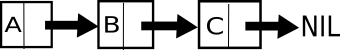
\includegraphics[width=9.0cm]{imgs/linked_list.png}
  \caption{Liste simplement chaînée.}
\end{figure}
En Lisp, une liste simplement chaînée peut être crée de la manière suivante. \\

\begin{lstlisting}[language=Lisp]
(defparameter *my-linked-list* '(1 2 3 4 5))
\end{lstlisting}
Ainsi, si nous reprenions le dessin que nous avions utilisé ci-dessus,
*my-linked-list* ressemblera donc à ceci: \\
\begin{figure}[H]
  \centering
  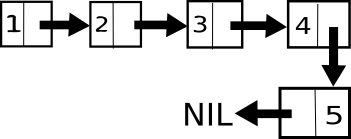
\includegraphics[width=9.0cm, height=2.5cm]{imgs/my_linked_list.png}
  \caption{*my-linked-list*}
\end{figure}
D'ailleurs, pour pouvoir travailler avec des listes chaînées, deux opérateurs bien pratiques s'offrent à nous: ``car'' et ``cdr''. \\[0.2cm]
\begin{lstlisting}[language=LISP]
CL-USER> (car *my-linked-list*)
1
CL-USER> (cdr *my-linked-list*)
(2 3 4 5)
\end{lstlisting}
Nous pouvons également chaîner nos opérateurs ``car'' et ``cdr'', afin de nous assurer un contrôle total sur notre liste simplement chaînée.
\begin{lstlisting}[language=LISP]
CL-USER> (car (cdr *my-linked-list*))
2
CL-USER> (cadr *my-linked-list*) ; Il existe aussi une manière abrégée.
2
\end{lstlisting}
Il existe également la fonction ``nth'', permettant de récupérer le n-ième élément d'une liste chaînée. (Il ne faut pas oublier que l'indexing marche comme pour les tableaux, et commence à 0.)
\begin{lstlisting}[language=LISP]
CL-USER> (nth 2 *my-linked-list*)
3
\end{lstlisting}

\subsubsection{Les tableaux.}
Le tableau est une structure extrêmement importante en programmation,
celle-ci nous permet de stocker un nombre fixe de données, et nous permet d'accéder à ces données de manière rapide. Chaque élément du tableau se retrouve collé en mémoire aux éléments qui lui sont adjacents, ainsi, pas besoin de traverser chaque élément du tableau lorsque l'on désire accéder au n-ième élément du tableau. \\[0.2cm]
Voici comment créer un tableau en Lisp:
\begin{lstlisting}[language=Lisp]
  CL-USER> (defparameter *my-array* #(1 2 3 4 5))
\end{lstlisting}
Il existe également une manière alternative:
\begin{lstlisting}[language=Lisp]
  CL-USER> (defparameter *my-array* (make-array 5 :initial-contents '(1 2 3 4 5)))
\end{lstlisting}
Pour récupérer le n-ième élément d'un tableau, il nous suffit de faire:
\begin{lstlisting}[language=Lisp]
  CL-USER> (aref *my-array* 2)
  3
\end{lstlisting}
\subsubsection{Tableaux vs Listes simplement chaînées.}
Pour en conclure avec ces deux structures de données, nous nous proposons de faire un petit tableau comparatif final, afin que le lecteur puisse mieux comprendre les différences entre Tableau, et Liste simplement chaînée, (que nous noterons SLL pour Single-linked list).
\begin{table}[H]
  \centering
  \begin{tabular}{|c|c|c|}
    \hline & Tableaux & SLL \\
    \hline {\bf Accession} & O(1) & O(n) \\
    \hline {\bf Insertion} & O(n) & O(1) \\
    \hline {\bf Délétion}  & O(n) & O(1) \\
    \hline
  \end{tabular}
\end{table} \smallskip
Comme on le constate sur ce tableau, les arrays ont un réel avantage lorsque nous désirons uniquement lire un élément de notre structure de données, toutefois, si nous désirons modifier la structure de données en elle-même, alors, tout devient plus problématique, et cela, car notre tableau devra retrouver un autre emplacement libre pour s'y mettre en mémoire. \\

La liste chaînée quant à elle, n'a pas besoin de se repositionner entièrement lorsqu'on lui ajoute ou qu'on lui retire un élément, il lui suffit plutôt de rajouter un pointeur vers le nouvel élément, ce qui se fait en temps constant (O(1)), peu importe la taille de la liste. Toutefois, la liste chaînée a pour inconvénient d'être en croissance linéaire lors de la recherche d'un élément dans la liste, en effet, lors de la recherche d'un élément dans une liste chaînée, le programme devra d'abord passer par tous les éléments se trouvant avant celui que l'on cherche. \\

Pour démontrer l'importance d'utiliser la bonne structure au bon endroit, nous allons reprendre notre bon tri à bulles. \\

Pour ceux qui avaient oublié l'implémentation sur les tableaux, la voici:
\lstinputlisting[language=Lisp]{Sorts/bubble_sort.lisp}
Le lecteur attentif remarquera l'utilisation dans ce code de ``make-array'' et de ``aref'', tout deux synonymes de l'utilisation d'un tableau. Maintenant, transformons cette implémentation en une implémentation utilisant des listes simplement chaînées. \\
Et maintenant, voici le même algorithme, mais, sur les listes simplement chaînées cette fois-ci.
\lstinputlisting[language=Lisp]{Sorts/bad_bubble_sort.lisp}
Et maintenant, comparons leurs temps respectifs sur des listes de tailles différentes avec l'aide d'un nouveau tableau, (notre mode opératoire reste le même, nous utilisons SBCL, et la macro time, pour créer une liste contenant des nombres aléatoires, nous utilisons toujours notre macro random-sample.)
\begin{table}[H]
  \centering
  \begin{tabular}{|c|c|c|}
    \hline & Tri à bulles (Tableaux) & Tri à bulles (SLL) \\
    \hline 10 &  0.0000008 secondes &  0.000009 secondes \\
    \hline 100 &  0.000089 secondes &  0.002111 secondes \\
    \hline 1000 & 0.007863 secondes &  0.750918 secondes \\
    \hline 10000 & 0.318904 secondes & 888.190640 secondes \\
    \hline 100000 &  31.164620 secondes & $>$1000 secondes \\
    \hline
  \end{tabular}
\end{table}
La différence de performance entre nos deux implémentations du même algorithme est énorme, et pourtant, nous n'avons pas changé l'algorithme en lui-même! J'espère que notre petite expérience montre bien au lecteur l'importance d'un choix de structure de données adéquat.
\subsubsection{Les tables de hachages.}
Une table de hachage (ou un dictionnaire en python) est une structure de données des plus utiles en ce qui concerne l'optimisation d'algorithmes. \\

Son utilisation est simple; avec une table de hachage, nous relions des clés avec des valeurs. \\

Ainsi, si dans une table de hachage, nous relions le mot ``bonjour'' avec le mot ``hello'', notre mot ``bonjour'' sera considéré comme étant la clé, et le mot ``hello'' comme étant la valeur. \\

En Lisp, pour créer une telle table de hachage, il faut faire: \\
\begin{lstlisting}[language=Lisp]
CL-USER> (defparameter *my-dict* (make-hash-table))
*MY-DICT*
CL-USER> (setf (gethash 'bonjour *my-dict*) 'hello)
HELLO
CL-USER> (gethash 'bonjour *my-dict*)
HELLO
\end{lstlisting}
Ce procédé étant toutefois un peu fastidieux, nous utiliserons ici la bibliothèque lisp connue sous le nom de serapeum. \\
\begin{lstlisting}[language=Lisp]
CL-USER> (ql:quickload :serapeum) ;; Ici, nous déclarons la bibliothèque.
To load "serapeum":
  Load 1 ASDF system:
    serapeum
; Loading "serapeum"
.
Switching to the BALLAND2006 optimizer

(:SERAPEUM)
CL-USER> (defparameter *my-dict* (serapeum:dict 'bonjour 'hello))
*MY-DICT*
CL-USER> (gethash 'bonjour *my-dict*)
HELLO
\end{lstlisting}
Pour montrer un cas pratique d'utilisation de tables de hachages, nous allons créer un mini-programme qui permet de convertir des phrases en morse. \\

Ce programme se fait en deux parties, tout d'abord, nous définissons une table de hachage qui nous remet la traduction morse de chaque lettre et de chaque chiffre. \\
\begin{lstlisting}[language=Lisp]
(ql:quickload :serapeum)

(defparameter *latin->morse*
  (serapeum:dict #\a "._" #\b "_..." #\c "_._." #\d "_.."
                 #\e "." #\f ".._." #\g "__." #\h "...."
                 #\i ".." #\j ".___" #\k "_._" #\l "._.."
                 #\m "__" #\n "_." #\o "___" #\p ".__."
                 #\q "__._" #\r "._." #\s "..." #\t "_"
                 #\u ".._" #\v "..._" #\w ".__" #\x "_.._"
                 #\y "_.__" #\z "__.." #\1 ".____" #\2 "..___"
                 #\3 "...__" #\4 "...._" #\5 "....." #\6 "_...."
                 #\7 "__..." #\8 "___.." #\9 "____." #\0 "_____"
                 #\SPACE " "))
\end{lstlisting}
Voici notre dictionnaire! Ne soyez pas surpris par les ``\#\'', c'est ainsi que nous définissons des caractères en common lisp. \\

Maintenant, la deuxième partie consistera simplement à créer une fonction chargée de transformer nos phrases en morse. \\
\begin{lstlisting}[language=Lisp]
(defun convert-to-morse (sentence)
  "Cette fonction s'occupe de convertir
nos phrases vers du code Morse, grâce au dictionnaire
créé ci-dessus!"
  (let ((converted-list
          (loop for letter across sentence
                collect (gethash letter *latin->morse*))))
  (format nil "~{~A~}" converted-list)))
\end{lstlisting}
Il ne nous reste plus qu'à tester.
\begin{lstlisting}[language=Lisp]
CL-USER> (convert-to-morse "ceci est une phrase")
"_._.._._... ...._ ..__.. .__......_.._...."
\end{lstlisting}
Et voilà comment notre programme marche! \\

Petite parenthèse au niveau de la complexité de notre fonction ``convert to morse''. Tout d'abord, il faut savoir que pour chercher une valeur avec une clé dans un dictionnaire, la complexité temporelle est de O(1)! Peu importe la taille du dictionnaire, cela prendra toujours aussi peu de temps de chercher une clef dedans, c'est la raison pour laquelle ceux-ci sont très utilisés de nos jours.
Pour les lecteurs intéressés, nous conseillons fortement de vous renseigner sur la fonction SHA, c'est grâce à cette fonction de hachage que les dictionnaires marchent aussi bien. \\

Ainsi, pour en revenir à notre programme, nous appliquons une opération de complexité O(1) sur chaque élément de notre liste, soit, n fois. On peut donc en déduire que notre fonction ``convert-to-morse'' est donc de complexité O(n), car nous appliquons n fois une opération de complexité O(1). \\[0.2cm]
\subsubsection{Promenons-nous dans les bois.}
Pour comprendre l'intérêt des arbres dichotomiques en programmation, intéressons nous à un petit problème assez simple. \\

Imaginez que je pense à un nombre, compris entre 1 et 1000, et que vous deviez deviner ce nombre avec le moins d'essais possible, à la même manière que dans le jeu du ``Juste Prix'', je vous dirai si votre essai est trop grand, ou trop petit. \\

La première stratégie évidente serait de commencer par 1; ensuite, si mon nombre n'est pas 1, essayer avec 2; puis, essayer avec 3, et ceci, jusqu'à ce que vous trouviez le nombre auquel je pense. \\

Cette première stratégie pourrait faire penser à la manière à laquelle il faut chercher un élément dans une liste simplement chaînée, en effet, si je pense au nombre 629, il va falloir passer par les 628-ièmes éléments se trouvant avant. Dans ce cas-ci, comme pour lire un élément dans une liste simplement chaînée, nous dirons que la complexité de cet algorithme sera de O(n). \\

Une deuxième manière de faire serait de faire ce que l'on appelle une recherche dite ``par dichotomie''. Tout d'abord, prenons un nombre au milieu entre 1 et 1000, ici, ce sera 500, si je dis ``au dessus'', alors, il suffira de prendre le milieu entre 500 et 1000, ici, ce sera 750, désormais, si je dis ``en dessous'', il faudra alors faire $\frac{500 + 750}{2} = 625$, ainsi, en appliquant cet algorithme jusqu'au bout, vous trouverez le nombre auquel je pense en utilisant un algorithme de complexité O(log n)! \\

Ainsi, vous trouverez grâce à cette technique le nombre auquel je pense en maximum $\log_{2}{n}$ essais (où n est le nombre maximum, qui est ici 1000). \\

J'espère que cette petite explication aura pu expliquer au lecteur le fonctionnement d'une recherche par dichotomie. Maintenant, pour ce qui est de l'implémentation d'une telle recherche en Lisp: \\
\lstinputlisting[language=Lisp]{LispBasics/dichotomia.lisp}
Plus qu'à la tester!
\begin{lstlisting}[language=Lisp]
[1] CL-USER> (binary-search 1 1000)
500?
plus-haut
750?
plus-bas
625?
plus-haut
687?
plus-bas
656?
plus-bas
640?
plus-bas
632?
plus-bas
628?
plus-haut
630?
plus-bas
629?
oui
Ton nombre a été trouvé en 9 essais
\end{lstlisting}

Cette petite introduction à la recherche par dichotomie servait surtout à donner une intuition au lecteur de l'importance des arbres binaires. \\

Ceux-ci fonctionnent d'une manière similaire à notre recherche dichotomique. \\

Sur un arbre binaire, chaque noeud est soit relié à rien (ou ``nil''), soit relié à sa ``gauche'' à un noeud contenant une valeur plus petite que celle de son noeud parent, soit relié à sa ``droite'' à un noeud contenant une valeur plus grande que celle de son noeud parent. Nous pouvons donc représenter un arbre binaire ainsi: \\

en lisp, pour définir un arbre binaire, nous ferons simplement:
\begin{lstlisting}[language=Lisp]
(defparameter *my-tree* '(10 (5 3 7) (15 (12 nil 14) (18 nil 20))))
\end{lstlisting}
Celui-ci sera représenté ainsi: \\
\begin{figure}[H]
  \centering
  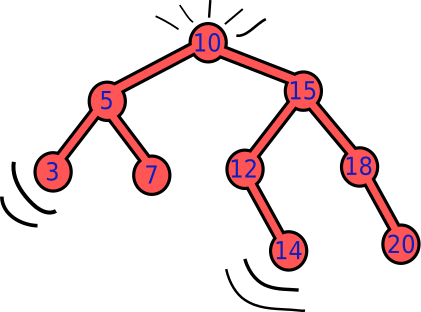
\includegraphics[width=8.0cm, height=5.5cm]{imgs/tree.png}
\end{figure}
\subsubsection{Les tas}
Nous faisons ci-dessous un petit aparté pour parler de tas. \\

Un tas n'est autre qu'une forme spéciale d'arbre où les valeurs sont ordonnées selon une certaine fonction ``clef''. \\

L'avantage du tas est avant tout que la complexité de la fonction pour récupérer l'élément au sommet du tas n'est autre que $O(1)$! \\

Un tas s'avère donc extrêmement pratique lorsque nous désirons garder des valeurs ordonnées, sans avoir à retrier la structure de donnée à chaque nouvel ajout de données. \\

Nous verrons comment utiliser les tas en Lisp dans la partie sur l'implémentation de l'algoithme A*.
\subsection{Qu'est-ce que Lisp?}
Lisp est une famille de langages de programmation fonctionnels, inventés en 1958 par John McCarthy (l'homme ayant inventé le terme ``intelligence artificielle''). \\

Ceux-ci sont reconnaissables facilement grâce au très grand nombre de parenthèses présentes dans chacun des dialectes de Lisp. \\

Aujourd'hui, le dialecte Lisp le plus utilisé reste {\bf Clojure}, toutefois, il en reste d'autres gardant toujours leur cote de popularité, pour n'en citer que quelques-un, nous avons
\begin{itemize}
  \item {\bf Scheme}, qui est un dialecte très minimaliste de Lisp, très utilisé au niveau académique.
  \item {\bf Emacs Lisp}, un dialecte très pratique pour tous ceux désirant configurer l'éditeur de texte Emacs.
  \item {\bf Racket}, un super-set de Scheme.
  \item {\bf Common Lisp} est le dialecte que nous utiliserons ici, ce dialecte a toujours eu la réputation d'être plus orienté vers les applications pratiques, et n'a jamais reçu de grandes faveurs académiques. Common Lisp a toutefois le mérite d'avoir été standardisé, de bénéficier d'un système orienté-objet connu sous le nom de CLOS.
\end{itemize}
\subsubsection{Les bases de Lisp.}
Tout d'abord, pour commencer notre aventure avec Lisp, ouvrons donc notre REPL (cela peut-être SBCL, Clisp, ou encore CCL), et additionnons deux nombres. \\
\begin{lstlisting}[language=Lisp]
CL-USER> (+ 3 5)
8
\end{lstlisting}
Cela peut sembler bien étrange pour le non-initié, et pourtant, tout cela est parfaitement logique. \\

En fait, lorsque l'on désire appeler une fonction (comme par exemple ici ``+''), la syntaxe sera toujours ``({\bf fonction} {\bf arguments})''. Prenons quelques autres exemples avec quelques opérations arithmétiques. \\
\begin{lstlisting}[language=Lisp]
CL-USER> (- 2 1)
1
CL-USER> (* 3 4 2)
24
CL-USER> (/ 5 6)
5/6
CL-USER> (/ 5 6.0)
0.8333333
\end{lstlisting}
Comme on peut le voir, la logique reste la même pour tous les opérateurs, aussi, cette syntaxe nous permet également de mettre à ces opérateurs autant d'arguments que l'on le souhaite, (l'exemple est donné ci-dessus avec l'opérateur de multiplication.). \\

Également, l'opération de division ne remet pas directement un nombre à virgule, mais plutôt un Ratio, si l'on ne lui donne pour argument uniquement des nombres entiers. \\

Pour déclarer une variable en Lisp, plusieurs choix s'offrent à nous, nous présenterons uniquement ici ``defparameter''.
\begin{lstlisting}[language=Lisp]
CL-USER> (defparameter *test* 'bonjour)
*TEST*
CL-USER> *test*
BONJOUR
\end{lstlisting}
J'en profite pour attirer l'attention sur l'utilisation de ``*'' autour du nom de la variable. Ceux-ci sont appelés les ``cache-oreilles'', il ne s'agit ici que d'une convention, il est tout à fait acceptable de ne pas utiliser de caches-oreilles lors de la définition d'une variable globale. \\

Maintenant, j'utiliserai la fin de cette petite introduction comme prétexte pour présenter ``la récursion''. \\

Pour montrer un exemple de fonction récursive, nous présenterons ici la fonction factorielle, fonction récursive par excellence. \\

Tout d'abord, pour déclarer une fonction, nous utiliserons le mot-clé {\bf defun}.
\begin{lstlisting}[language=Lisp]
CL-USER> (defun factorial (x) ...)
\end{lstlisting}
Il faut ensuite réfléchir à ce qu'il faudra mettre au sein de notre fonction. \\

La récursion est un processus en 3 étapes. \\
\begin{enumerate}
  \item Trouver la valeur de f(0) (ou de n'importe quel cas de base.)
  \item Supposer que cette fonction remettra un nombre correct pour f(n-1).
  \item Trouver la valeur de f(n) en fonction de f(n-1).
\end{enumerate}
L'exemple ici est assez simple, et est souvent donné en introduction à la récursion. Voici donc une définition formelle de notre fonction factorielle. \\
$$\begin{cases}0! = 1 \\ n! = n \cdot (n - 1)! \end{cases}$$
Ainsi, uniquement grâce à cette simple définition, nous allons pouvoir coder cette fonction en Common Lisp \\
\begin{lstlisting}[language=Lisp]
CL-USER> (defun factorial (x)
                   (if (= x 0)
                       1
                      (* x (factorial (- x 1)))))
FACTORIAL
\end{lstlisting}
On constate directement la simplicité et l'élégance avec laquelle cette fonction peut être ainsi programmée. D'autres fonctions peuvent-être codée de manière récursive, l'exemple de l'algorithme de tri par fusion, ou encore l'agorithme d'Euclide pour calculer le pgcd sont deux exemples de fonctions récursives dont j'ai pu montrer l'implémentation ci-dessus. \\

Un autre exemple d'algorithme utilisant la récursion serait l'algorithme ``quick-sort'' dit du ``tri-rapide'', en voici son implémentation \\

\lstinputlisting[language=Lisp]{Sorts/quick_sort.lisp}
Si le lecteur en sent l'envie, nous l'encourageons à essayer de coder la fonction récursive d'Ackermann, ou encore la McCarthy 91. \\
\subsubsection{Métaprogrammons!}
Cette petite partie a pour objectif de montrer en quoi Lisp est si bon: {\bf La métaprogrammation}!
La métaprogrammation, c'est l'art de faire des programmes qui manipulent le code du programme même!\\

Passons directement aux exemples:\\

En Common Lisp, il est possible de créer des variables locales avec l'aide du mot-clé {\bf let}. Par exemple, si nous désirions créer de manière non récursive la fonction: \\

$$f(n) = \sum_{i=0}^{n}i$$
Nous devrions faire: \\
\lstinputlisting[language=Lisp, linerange={1-5}]{LispBasics/sum.lisp}
Toutefois, certains ne trouvent pas très esthétique le fait de devoir empiler des parenthèses à chaque fois qu'un très petit {\bf let} est appelé. \\

Pour remédier à cela, il est possible de modifier la manière à laquelle notre code Lisp est lu! \\

Ainsi, en créant la macro: \\
\lstinputlisting[language=Lisp, linerange={7-9}]{LispBasics/sum.lisp}
Il devient possible de modifier notre fonction de base: \\
\lstinputlisting[language=Lisp, linerange={11-15}]{LispBasics/sum.lisp}
Tout de suite, le code devient (pour certains) plus agréable à lire.\\

En réalité, notre nouvelle fonction est exactement la même que l'ancienne! La macro que nous avions créée se fait remplacer par le préprocesseur.
\begin{lstlisting}[language=Lisp]
CL-USER> (macroexpand '(let-in buffer 10 (+ buffer 5)))
(LET ((BUFFER 10))
  (+ BUFFER 5))
\end{lstlisting}
Le code ci-dessus illustre la manière à laquelle le préprocesseur évalue notre macro.\\

Un autre exemple de macro sont les Reader Macros, celle-ci ont pour objectif de complètement modifier la syntaxe même de Common Lisp. \\

Un exemple de Reader Macro, serait par exemple une pour créer des lambdas de manière plus simple:\\

Sans plus attendre, voici la macro: \\
\lstinputlisting[language=Lisp]{LispBasics/reader.lisp}
Et voici comment elle s'utilise: \\
\begin{lstlisting}
CL-USER> (mapcar <1+ (* 2 _)> '(1 2 3 4))
(3 5 7 9)
CL-USER> (macroexpand '<1+ (* 2 _)>)
#'(LAMBDA (_) (1+ (* 2 _)))
T
\end{lstlisting}
Le lecteur intéressé pour s'essayer au fonctionnement des macros anaphoriques, qui ne sont pas présentées dans cette introduction.\\
\subsubsection{Programme Lisp pour résoudre parfaitement le jeu de Nim.}
Afin que le lecteur se fasse une idée de comment utiliser Lisp dans des cas plus concrets, nous allons vous présenter une intelligence artificielle, assez basique, gagnante au jeu de Nim à plusieurs tas. (Aussi connu sous le nom de jeu de Marienbad.), dans ce jeu, plusieurs allumettes sont disposées sur plusieurs piles, le but du jeu est de récolter la dernière allumette. \\

L'intelligence gagnante à ce genre de jeux est assez basique, en effet, le jeu de Nim à plusieurs tas est un jeu résolu parfaitement. \\

La stratégie gagnante pour ce jeu est simple, nous définissons une position gagnante une position où la``nim-somme'' (qui est en réalité l'opérateur ``xor'' ou $\oplus$ appliqué à la représentation binaire de notre tas) est différent de 0, et à l'inverse, une position perdante est une position où la ``nim-somme'' appliquée aux tas est égale à 0. \\

Un exemple de position perdante serait la position où les allumettes seraient réparties sur 4 tas avec 1 allumette sur le premier tas, 3 sur le deuxième, 5 sur le 3ième, et 7 sur le dernier. \\
$$1 \oplus 3 \oplus 5 \oplus 7 = 0$$
Pour se le prouver, on peut utiliser notre interprète Lisp et faire
\begin{lstlisting}[language=Lisp]
CL-USER> (logxor 1 3 5 7)
0
\end{lstlisting}
Le but de l'ordinateur sera donc de toujours se trouver en position de sécurité, et de toujours mettre le joueur en position perdante. \\

Le twist que nous avons apporté est le fait que le joueur peut décider des tas avec lesquels ils va jouer, et ainsi, mettre directement l'ordinateur en position de défaite, notre IA devra donc se montrer capable de jouer des coups, même en perdant. \\
\lstinputlisting[language=Lisp, linerange={1-2}]{Nim/nim-game-player.lisp}
Ici, nous ne faisons que définir une variable globale *heaps*, celle-ci représentera les tas disponibles au travers de notre programme. \\
\lstinputlisting[language=Lisp, linerange={4-10, 27-32, 61-67}]{Nim/nim-game-player.lisp}
Ces deux fonctions seront dites des ``fonctions d'aide'', elles auront surtout pour utilité de ne pas avoir à surcharger les fonctions principales. \\

Le lecteur attentif remarquera que nous terminons le nom de ces fonctions par un ``p'', cela est dû au fait que ces fonctions sont des {\bf prédicats}, elles ne peuvent retourner que ``t'' ou ``nil'' (``vrai'' ou ``faux''), ceci n'étant également qu'une convention, si le lecteur désire écrire des prédicats sans laisser de ``p'' au bout, SBCL ne lui trouvera rien à redire.\\

Aussi, on peut remarquer dans les deux premières fonctions l'utilisation de ``reduce'', il s'agit d'une fonction destinée aux {\bf catamorphismes}, cela veut dire qu'elles permettent de passer d'une structure de données comme une liste, ou un arbre, vers un scalaire, comme un entier ou encore un flottant. \\

Egalement, j'utilise \# , ce symbole nous permet d'expliciter que nous utilisons une fonction, et pas une variable.\\
\lstinputlisting[language=Lisp, linerange={12-26, 34-48}]{Nim/nim-game-player.lisp}
Nous voici enfin au cœur du programme. Avec nos fonctions ``play-winning-move'' et ``play-random-legal-move'' qui sont nos deux fonctions où est contenu notre joueur, les commentaires explicitant déjà leurs actions, nous nous concentrerons surtout sur l'implémentation. \\

Comme nous le remarquons, j'utilise {\bf let} et {\bf loop}, {\bf let} me permet de déclarer des variables dites ``locales'', cela me permet d'avoir un code propre, où chaque chose reste à sa place. \\

{\bf loop} est une macro, qui permet d'itérer, ou de répéter un nombre certain de fois une même action, nous l'utilisons ici en raison de la lisibilité de celle-ci, certains préfèrent la macro ``do'', nou trouvons cette dernière illisible, mais nous encourageons le lecteur à se renseigner sur cette dernière si le coeur lui en dit.\\
\lstinputlisting[language=Lisp, linerange={50-60}]{Nim/nim-game-player.lisp}
Nous ne ferons remarquer ici que l'utilisation de la macro {\bf cond}, une autre manière d'écrire des conditions en Lisp.
\lstinputlisting[language=Lisp, linerange={69-95}]{Nim/nim-game-player.lisp}
Cette très longue fonction fait office d'interface utilisateur. Nous avons déjà fait remarqué au lecteur en commentaires l'utilisation de la récursion. \\

Egalement, nous signalons {\bf progn}, une fonction bien pratique pour définir des blocs de code.
\lstinputlisting[language=Lisp, linerange={98-108}]{Nim/nim-game-player.lisp}
Nous finissons enfin notre programme avec cette fonction nim-game-repl, permettant de commencer une partie entre humain et ordinateur.
\subsection{Le pathfinding.}
Le ``pathfinding'' (ou la ``recherche de chemin'' en français) est un ensemble de problèmes dans le domaine de l'intelligence artificielle où l'objectif est de trouver le chemin optimal entre deux points dans un graphe. \\
\subsubsection{Présentation du problème.}
Ici, le problème que nous allons essayer de résoudre est de trouver le chemin optimal entre deux villes belges. \\

Les villes belges que nous utilisons ici sont répertoriées dans le document CSV présent à l'adresse suivante: \url{https://github.com/spatie/belgian-cities-geocoded},
comme vous le constatez, ce fichier fait plus de 2500 éléments, il va donc falloir être judicieux dans le choix des structures de données, et des algorithmes utilisés afin d'espérer avoir une implémentation un minimum correcte. \\[0.2cm]
\subsubsection{L'algorithme de Dijkstra.}
Cet algorithme de recherche, inventé par Edsger Dijkstra dans les années 50, marche de la manière suivante: \\

Tout d'abord, pour représenter l'espace dans lequel notre algorithme doit chercher, nous utiliserons un graphe avec des poids, en voici un exemple: \\
\begin{figure}[H]
  \centering
  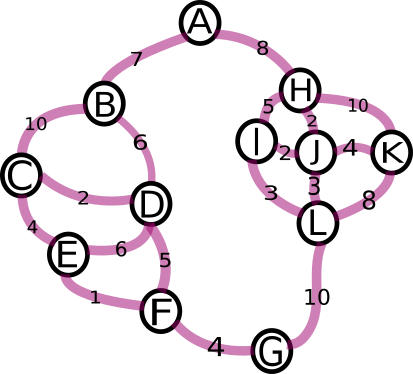
\includegraphics[width=8.0cm]{imgs/numbered_graph.png}
  \caption{Graphe avec poids.}
\end{figure}
Ainsi, imaginons que nous cherchons le chemin optimal entre la ville A et la ville G. Nous allons entreprendre les recherches avec l'aide de l'algorithme de Dijkstra. \\

Cet algorithme se déroule en plusieurs parties, tout d'abord listons l'ensemble des villes joignables directement depuis notre première ville. \\

Dans notre graphe ci-dessus, les villes B et C sont directement accessible via A.\\

Voici les chemins marqués sur le graphe : \\
\begin{figure}[H]
  \centering
  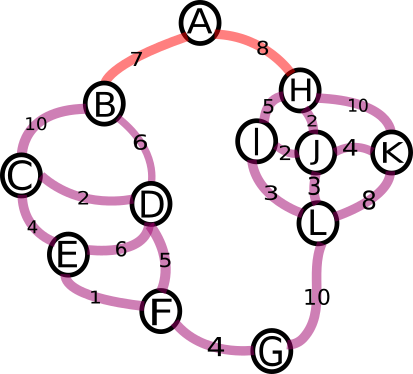
\includegraphics[width=8.0cm]{imgs/second_search.png}
\end{figure}
Ainsi, nous pouvons créer une file des priorités, reprenant les villes visitées et les triant en fonction du coût nécessaire pour y accéder (cette file des priorités sera implémentée avec l'aide d'un tas). \\
\begin{itemize}
  \item Pour B, ce coût sera de 7.
  \item Pour H, ce coût sera de 8.
\end{itemize}
Il faut donc visiter en priorité la ville B! \\

À partir de B, nous pouvons visiter les villes D et C, voici les chemins empruntés: \\
\begin{figure}[H]
  \centering
  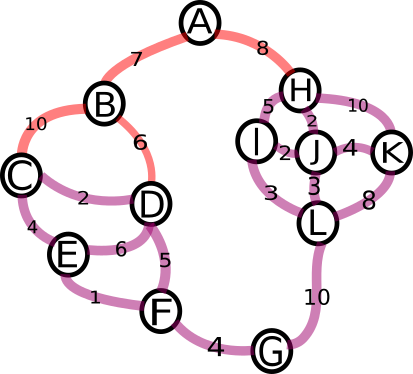
\includegraphics[width=8.0cm]{imgs/third_search.png}
\end{figure}
Nous pouvons désormais mettre à jour notre liste des priorités en retirant B, et en y rajoutant: \\
\begin{itemize}
  \item C avec un coût de 7 + 10 = 17
  \item D avec un coût de 7 + 6 = 13
\end{itemize}
Notre liste des priorités sera ainsi composée dans l'ordre de H, puis de D, puis de C. \\

Il faudra donc visiter la ville H! \\

De H, nous pouvons visiter les villes I, J et K, voici encore une fois le graph des villes visitées : \\
\begin{figure}[H]
  \centering
  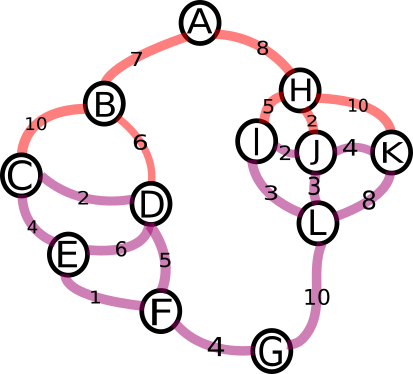
\includegraphics[width=8.0cm]{imgs/fourth_search.png}
\end{figure}
Nous rajoutons ainsi à notre liste des priorités ces villes avec les coûts associés : \\
\begin{itemize}
  \item I avec un coût de 8 + 5 = 13
  \item J avec un coût de 8 + 2 = 10
  \item K avec un coût de 8 + 10 = 18
\end{itemize}
Il faudra donc visiter en priorité J ! \\

Il faut ainsi répéter les étapes de cet algorithme, jusqu'à obtenir la solution finale: le chemin optimal ! \\

Le lecteur pourra s'essayer à trouver le chemin optimal entre A et G, en appliqant scrupuleusement l'algorithme de Dijkstra, le graph montrant le chemin optimal sera présenté à la page suivante.
\begin{figure}[!hbt]
  \centering
  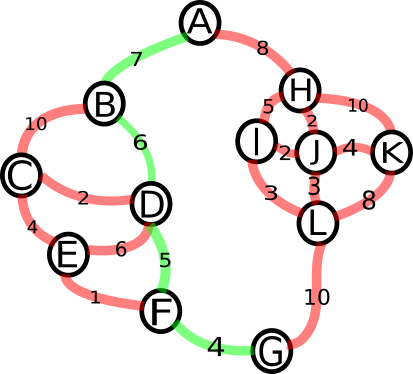
\includegraphics[width=8.0cm]{imgs/solved.png}
  \caption{Le chemin optimal!}
\end{figure}
Toutefois, on remarque vite un problème avec cet algorithme: toutes les villes ont du être visitées afin de pouvoir résoudre correctement notre problème! \\

Cela ne peut pas sembler être bien grave sur un si petit exemple, mais, quand il s'agit d'effectuer cet algorithme sur toutes les villes belges, il devient clair que nous avons une perte en performances.\\

Il va donc falloir ruser, et utiliser une heuristique afin d'avoir de meilleurs temps, et espérer pouvoir appliquer notre algorithme raisonnablement sur l'ensemble des villes belges. \\

Ces methodes d'heuristique seront justement discutées dans le prochain chapître à leur sujet. \\
\subsubsection{Le besoin d'heuristiques.}

Dijkstra a l'avantage d'être un algorithme donnant toujours la solution optimale, ainsi, peu importe le graphe dans lequel nous appliquons notre algorithme de Dijkstra, le chemin trouvé entre deux points de notre graph sera toujours le plus optimal. \\

En contrepartie, cet algorithme a pour défaut de bien souvent visiter un nombre assez important de noeuds sur notre graphe, ceci ayant pour conséquence de baisser la performance de notre algorithme. \\

Fort heureusement, des mathématiciens ont trouvé une solution afin de remédier à ce problème: {\bf Créer une heuristique!} \\

Une heuristique est un outil nous permettant de prendre des décisions, de faire des choix. Une heuristique intéressante dans le cadre de notre problème avec un algorithme de Dijkstra, serait de privilégier uniquement certains noeuds nous rapprochant de la solution finale. \\

Il faut toutefois faire attention dans le choix de notre heuristique,
une mauvaise heuristique pourrait nous faire retirer trop de noeuds d'une solution potentielle, et ainsi, produire des solutions sous-optimales. \\
\subsubsection{Dijkstra avec de l'heuristique: A*!}
L'algorithme A* est un algorithme de Dijkstra avec une heuristique intéressante. \\

Ainsi, pour chaque noeud de notre graphe, nous allons-y rajouter un ``coût'' heuristique. Celle qui sera choisie ici sera la distance euclidienne entre le noeud du graphe et l'objectif final. \\
Afin d'illustrer nos propos, nous avons ci-dessous implémenté l'algorithme A*.
\pather{1-2}
Tout d'abord, les deux librairies que nous utiliserons ici seront ``cl-csv'', similaire à pandas de python, cette librairie permet de traîter les fichiers csv (comma-separated values). \\

La seconde est serapeum, cette bibliothèque, au même titre que alexandria, permet d'étendre Common Lisp, afin d'en faire un outil bien pratique, nous nous servons de serapeum avant tout pour pouvoir utiliser les tas que cette librairie nous offre.
\pather{7-25}
Ici, nous reprenons simplement les données du CSV de belgian-cities-geocoded et les entrepose dans un très grand tableaun, ici *belgian-cities*. Le lien du CSV est donné dans le doc-string accompagnant le paramètre global.
\pather{4-5}
{\bf defstruct} permet de créer des structures Common Lisp, il est possible de voir celles-ci comme les namedtuples de la bibliothèque collections de python.
\pather{28-53}
Ces deux fonctions permettent de calculer la distance entre deux villes en fonction de leur latitude et de leur longitude. La formule permettant de faire cela s'appelle ``formule de Haversine''\footnote{https://fr.wikipedia.org/wiki/Formule\_de\_haversine}.
\pather{55-62}
Cette fonction prend une ville en argument, et retourne chacune des villes se trouvant à un rayon de 20km de celle-ci. \\

On peut remarquer l'utilisation d'un {\bf remove-if}, cette fonction d'ordre supérieur filtre tous les éléments d'une structure de données ne respectant pas un certain prédicat.
\pather{64-69}
Comme expliqué dans le docstring, cette fonction a pour objectif d'affecter une priorité à chaque élément du tas, en fonction du coût heuristique et du coût réel. \\

Il est intéressant de noter que pour réaliser un algorithme wA*, la seule modification à faire au programme est de modifier {\bf heuristic-comp} en
\begin{lstlisting}[language=Lisp]
(defun weighted-heuristic (city weight)
   (- 0 (+ (* weight (city-heuristic city))
            (city-cost city))))
\end{lstlisting}
Passons aux trois prochaines fonctions:
\pather{71-85}
Celles-ci n'ont malheureusement pas grand chose de très intéressant,
elles ont été crées afin de limiter la taille du programme, et de rendre le code propre, \\

Il est toutefois intéressant de s'intéresser à for-it-over, qui est une macro anaphorique, cela veut dire que celle-ci se permet de garder le résultat des calculs effectués à l'intérieur dans une variable, passant celle-ci au reste du programme. \\

Les macros anaphoriques sont toutefois à doubles-tranchants, bien qu'elles puissent faire gagner un programme en élégance, elles ont le don de faire en sorte que le lecteur s'y perde, et ne comprenne pas d'où proviennent les variables ``it'' se promenant librement dans le programme sans avoir été déclarées explicitement.
\pather{89-130}
Et enfin, voici l'algorithme A* en lui même! \\

Remarquons l'utilisation assez forte de ``loop'', donnant un style assez impératif à cette implémentation. \\

Il s'agti d'ailleurs d'un avantage de Lisp, le langage est multiparadigme, et permet de coder de la manière à laquelle l'utilisateur le souhaite! \\
\subsection{Des programmes et des jeux!}
Dès les débuts de l'intelligence artificielle, une envie de battre des humains avec des ordinateurs à des jeux de société s'est fait sentir. \\

Un exemple historique de cela est la défaite de Kasparov face à Deep Blue d'IBM.\\

Le but de ce chapître est de présenter comment un ordi peu gagner contre un humain à un jeu de société, et quelles stratégies doivent être appliquées.\\

Nous implémenterons une IA capable de battre un humain à puissance 4.\\
\subsubsection{L'agorithme Minimax.}
À la base de cette section se trouve l'algorithme minimax. Pour comprendre celui-ci, nous allons jouer à un jeu!\\
Prenons comme plateau l'arbre suivant:
\begin{figure}[H]
  \centering
  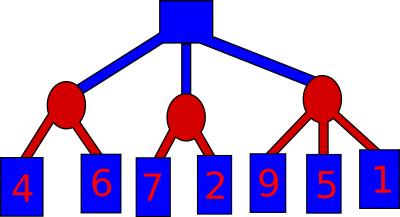
\includegraphics[width=8.0cm]{imgs/minimax_start.png}
\end{figure}
Le but du jeu est simple: \\

À chaque case bleue sur laquelle nous nous trouvons, vous avez le droit de déplacer le joueur où vous le voulez, dès que nous sommes sur une case rouge, c'est à notre tour de déplacer le joueur!\\

Votre but est d'atterrir sur la case la plus grosse possible, le mien est de vous faire atterrir sur la case détenant la plus petite valeur possible.\\

Comme première stratégie, vous pourriez être alléché par le 9, et vous déplacer directement vers la case rouge permettant d'y accéder. \\

Le défaut de cette stratégie est que si vous désiriez appliquer cette stratégie, alors, nous déplacerions simplement le joueur vers le 1, et vous vous retrouveriez avec le pire résultat possible.\\
Il va donc falloir innover.\\

La stratégie du minimax consiste à dire que nous jouerons à chaque fois le coup le plus minimisant, et ainsi, il est possible de remplacer chacun de mes choix par la valeur de la case la plus petite qui me serait accessible depuis la case où nous nous trouvons.\\

Ainsi, nous pourrions représenter notre plateau ainsi:\\
\begin{figure}[H]
  \centering
  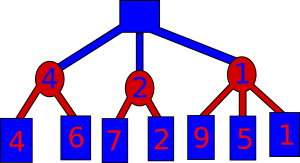
\includegraphics[width=8.0cm]{imgs/minimax.png}
\end{figure}
De cela, il devient très clair que le meilleur score que vous puissiez espérer avoir est 4.\\

Ainsi, c'est par une alternance de cycle où l'on minimise les scores, et de cycles où on les maximise que se déroule le minimax (en effet, si nous devions prédire votre coup, nous dirions que vous iriez toujours vers là où la case est la plus haute.)\\

Le défaut du minimax est quand le nombre de positions dans la partie devient énorme. C'est le cas du puissance 4, ou encore du jeu d'échecs, il faut donc pouvoir construire des heuristiques ou alors poussez l'optimisation jusqu'au bout.\\

Le reste de ce chapître présente quelques méthodes d'optimisations de l'algorithme minimax.\\
\subsection{Un programme de jeu.}
Nous voici enfin au cœur du sujet, avec l'implémentation de notre algorithme Minimax en Common Lisp. Le code se sépare en trois parties:
\begin{enumerate}
  \item La partie Logique de Jeu
  \item La partie Minimax
  \item La partie interface utilisateur
\end{enumerate}
sans plus tergiverser, analysons de suite le code.
\connect{1-7}
Ici, nous utilisons deux variables globales, toujours en respectant la convention des cache-oreilles. Il est intéressant de noter qu'il est en général conseillé de limiter le nombre de variables globales se promenant dans un code au strict minimum, en effet, celles-ci empêchent une lecture linéaire, et peuvent mener à ce qui est connu sous le nom de ``code spagetthi''. Dans notre code de puissance 4, nous n'en utiliserons au total trois.
\connect{9-14}
Avec cette fonction permettant de construire un nouveau tableau, nous entamons notre première partie concernant la logique de jeu. \\

Il est intéressant ici de noter la structure de donnée représentant le tableau de jeu. Un tableau comprenant des listes simplement chaînées. Nous avons choisi une structure de donnée si originale simplement car nous aimions la manière à laquelle celle-ci se laissait représenter en mémoire. \\
\connect{16-39}
{\bf count-to} et {\bf playerify} servent juste à alléger la syntaxe à certains endroits.
Nous faisons remarquer avant tout l'utilisation de {\bf gensym} dans notre macro, {\bf gensym} a pour rôle de créer un symbole au nom unique, ainsi, les variables étant définies dans la macro ne peuvent pas être appelées en dehors de la macro ({\bf gensym} existe également en prolog). {\bf case} est l'équivalent de {\bf switch} en C. \\

{\bf show-board} nous permet d'afficher notre structure de donnée à l'écran de manière convenable.
\connect{41-53}
Voici trois fonctions d'aide, celles-ci ont pour but d'alléger grandement le corps des fonctions plus grandes, se situant plus loin dans le code. Nous recommandons grandement la lecture de {\bf The Little Schemer} afin de comprendre pourquoi de telles fonctions sont très importantes.

\connect{55-67}
Notons ici l'utilisation de {\bf \&optional}, permettant d'utiliser des paramètres optionnels. Et {\bf labels} permettant de définir des fonctions à l'intérieur d'autres fonctions.

\connect{70-90}
Encore deux fonctions d'aides, celles-ci seront très pratiques pour vérifier le nombre de connections entre les jetons sur notre plateau de puissance 4.

\connect{92-114}
Ici, nous définissons enfin des fonctions permettant de vérifier le nombre de connections verticales et horizontales sur notre plateau. Attention au faux-amis! {\bf return} en Common Lisp n'est utile que dans les boucles, pour retourner une valeur à partir d'une fonction, il n'est nécessaire de préciser return que lorsque nous désirons faire sortir une valeur d'une boucle.\\

Le code pour vérifier les connections horizontales et verticales reste relativement simple. Intéressons-nous maintenant au code permettant de vérifier les connections en diagonale.

\connect{117-174}
Ici, remarquons la définition de constantes. Les constantes sont à différencier des variables globales telles que *moves* de par le fait qu'elles sont parfaitement immutables, et ainsi, plus facilement optimisables par le compilateur et laissent au code sa lisibilité. \\

L'utilisation d'une macro dans le cas de {\bf max-in-some-diagonal} aurait put être remplacé par une simple fonction d'aide. Nous aimions juste la liberté supplémentaire au niveau de la syntaxe dans la définition des fonctions du dessous que nous offrait la macro.

\connect{176-188}
Voici enfin les deux dernières fonctions composant notre partie de la logique de jeu. {\bf connections} est encore une fois une fonction d'aide, il est intéressant de noter ici l'utilisation de {\bf max} comme fonction polyvariadique.

\connect{190-205}
Notre partie Minimax commence enfin avec la fameuse fonction d'évaluation. Celle-ci marche avec la formule suivante:
$$eval = 1R * 1 + 2R * 550 + 3R * 3500 + 4R * 50000000 - 1Y * 1 - 2Y * 550 -3Y * 3500 - 4Y * 50000000$$
Celle-ci est bien évidemment perfectible, (lors des scéances de tests, celle-ci apporta à notre algorithme un comportement fort sadique).

\connect{207-257}
Toutes les fonctions suivantes ne sont que des fonctions d'aide, nous n'allons pas tergiverser énormément dessus. La chose importante à noter toutefois est l'utilisation de {\bf (declaim (inline f))} permettant de définir une fonction comme étant inline (il s'agit simplement d'une technique d'optimisation, les fonctions inlines étant en dehors de la portée de ce projet, nous encourageons le lecteur à se renseigner sur celles-ci de lui-même).

\connect{259-275}
Ces fonctions permettent de créer un tableau de puissance 4, uniquement en fonction d'une suite de coups. {\bf flet} a la même fonction que {\bf labels}.

\connect{277-283}
Deux fonctions d'aide, leur intérêt est assez explicite grâce aux doc-strings les accompagnants.

\connect{291-327}
Voici enfin venir la fin de notre partie minimax. \\

Nous nous intéresserons ici à l'intérêt de {\bf multiple-value-bind}, en effet, en Lisp, il est possible de retourner plusieurs valeurs d'une fonction grâce à l'utilisation de {\bf values}. Il faut tout de même un moyen de récupérer toutes les valeurs sorties de la fonctions, et savoir relier ses valeurs à des variables. C'est ici qu'entre en jeu {\bf multiple-value-bind}, dont l'intérêt est justement de récupérer les valeurs sorties par {\bf values} et les rattacher à des variables locales.

\connect{329-363}
Voici en fin venir la fin du programme Lisp, avec la partie interface utilisateur, le programme permet de jouer contre un autre joueur, ou encore de jouer contre l'IA. \\
\subsubsection{$\alpha\beta$-élagage.}
L'alpha-bêta élagage est une technique d'optimisation inventée par nul autre que John McCarthy (l'inventeur du Lisp, en personne!).\\

Nous ne rentrerons pas dans les détails du fonctionnement de l'$\alpha\beta$-élagage. En clair, celui-ci permet de réduire grandement le nombre de recherches à faire dans l'arbre de décision sur lequel nous appliquons notre algorithme minimax.\\

En effet, il n'est pas nécessaire de visiter les positions où l'évaluation n'est pas assez favorable.\\

L'arbre de jeu étant tellement énorme, il est extrêmement pratique de ne pas avoir à tout visiter.
\subsubsection{Du dynamisme bon sang !}
Le principe de la programmation fondateur dynamique est assez simple: Il est plus facile de mémoriser que de calculer.\\

La programmation dynamique se base sur le principe du Divide and Conquer (ou ``diviser pour mieux régner'' en français). Il faut tout d'abord répartir le problème en plusieurs petites tâches plus simples à résoudre, par la suite, nous stockons les résultats intermédiaires, et grâce à ces résultats stockés, nous pouvons arriver à une solution finale plus rapidement que si nous devions à chaque fois tout recalculer à partir de 0.\\

Nous utiliserons une stratégie s'appelant la {\bf mémoization} afin d'optimiser notre algorithme du Minimax.\\
La {\bf mémoization} est une stratégie typique en programmation fonctionnelle.\\

Le principe est simple: Chaque fois que nous appelons une fonction, nous stockons le résultat associé à la valeur entrée dans une table de hachage, dès que nous rappelons la fonction, nous vérifions si le paramètre de celle-ci se trouve dans notre table de hachage.\\
Si c'est le cas, nous retournons directement la valeur associée à la clé, n'oublions pas que cette opération est de complexité O(1), ce qui explique l'intérêt de stocker le résultat plutôt que d'avoir à le recalculer entièrement.\\

Nous utilisons cette stratégie dans notre puissance 4 avant tout car il est possible d'atteindre une même position, à partir de suites de coups différentes, il est donc intéressant de ne pas avoir à réévaluer la position inutilement.
\newpage
\section{Le Machine Learning.}
\subsection{Définition du Machine Learning}

Le Machine Learning, ou Apprentissage Automatique, est un type d'intelligence artificielle qui analyse et s'entraine avec des données, permettant dès lors aux ordinateurs d'apprendre par expérience (sans avoir été explicitement programmé à cet effet ou par intervention humaine). Cela consiste en algorithmes d’apprentissage qui améliorent leur performance à exécuter des tâches au fil du temps grâce à de l’expérience.\\

Le machine learning est présent dans la vie de tous les jours. Par exemple, nos boîtes mail sont équipées d'algorithmes capables d’apprendre avec le temps. Prenons les spams, leurs émetteurs sont capables de s'adapter, de changer leur manière d’agir, il est donc impératif que l’algorithme de défense contre les spams change lui aussi. Dans les e-mails, le machine learning se cache aussi derrière les réponses automatiques, en 2018, 6,7 milliards des mails envoyés étaient des réponses automatiques. On peut aussi trouver des IA dans les réseaux sociaux (reconnaissance faciale entre amis Facebook,...), blocage automatique des cartes de crédit volées, et bien d'autres.\\

\subsection{Les Maths dans le Machine Leanring.}

De nombreux data scientists (chargés de la gestion, de l’analyse et de l’exploitation des données au sein d’une entreprise) considèrent le machine learning comme un apprentissage statistique car celui-ci s’appuie sur des algorithmes (principalement statistique) permettant à une machine d'apprendre grâce à des échantillons ou bases d’apprentissages.\\

Ce qu’on appelle machine learning est pour certains la rencontre des statistiques avec la puissance de calcul disponible aujourd’hui (mémoire, processeurs, cartes graphiques).\\

On retrouve aussi dans le machine learning; les fonctions, elles sont utiles à l’analyse des séries temporelles (suite de valeurs numériques représentants l’évolution d’une quantité spécifique au cours du temps), les variables, les équations, les graphiques, et d’autres outils mathématiques de ce genre.\\[1cm]

Il existe beaucoup d'algorithmes diffèrents qui sont utilisés dans le machine learning. Ici, quelques exemples seront donnés mais seulement un sera expliqué.\\

"L'arbre de décision", celui-ci sert à classifier une série de donné futur grâce à des données déjà connue. Petit exemple par rapport à l'acceptation d'un crédit bancaire ; 2201 clients au départ dont 1427 cibles (dont le crédit a été accepté), 774 non-cible(crédit refusé). La variable séparant le mieux les dossiers est l'âge du client. Ensuite, en observant mieux, il est possible de remarquer que chez les 18 à 42 ans, le taux d'acceptation est plus élevé, mais est surtout accepté aux personnes ayant des revenus supérieurs à 55 k euros. Pour les 43 à 62 ans, le sexe est la variable la plus explicative, les femmes ont un taux d'acceptation plus élevé que les hommes. Enfin, pour les plus de 63 ans, le taux d'acceptation de crédit est très faible et ne dépend plus d'autre variable, car l'âge pour eux est déjà la variable la plus explicative.\\

\begin{figure}[H]
  \centering
  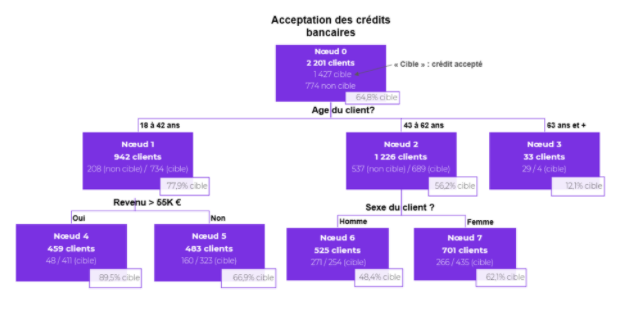
\includegraphics[scale=1]{imgs/algo_ml.png}
\end{figure}

"Les Forêt Aléatoires", le "Gradient Boosting"/"Xg Boost", "les algorithmes génétiques", les "machines à vecteurs de support", les "k plus proches voisins",... sont tous des algorithmes utilisés en Machine Learning.

\subsection{Les résaux de neurones}
Une couche de neurones d’entrées, plusieurs couches cachées, une couche de sortie suivie d’une fonction d’activation.
Chaque neurone possède une valeur obtenue par une fonction de combinaison étant la somme des valeurs des neurones de la couche précédente, chacune multipliée par un poids spécifique
$ z = x_1 \cdot p_1 + x_2 \cdot p_2 + \cdots + x_n \cdot p_n $ \\

Une fois la (ou les) valeur(s) de la couche de sortie obtenue, on applique à celle-ci une fonction d’activation qui transforme la valeur en fonction d’un seuil. Si en dessous du seuil, inactif (0/-1), aux environs du seuil, phase de transition, et au-dessus du seuil, actif (1/$>$1). Le type de fonction varie d’un cas à l’autre, mais les plus récurrentes sont la fonction sigmoïde $ \frac{1}{1 + e^{-x}} $ la fonction tangente hyperbolique $ \frac{2} {1 + e^{-2x}} -1 $
ou encore la fonction ReLU $ \begin{cases} 0 & x < 0 \\ x & x >= 0 \end{cases} $ \\

Durant l’apprentissage, les poids sont des valeurs prises au hasard. Il faut donc les ajuster pour fournir une réponse qui se rapproche au mieux de la réalité. Comme on entraîne notre réseau, on connaît la vraie valeur finale. On va donc appliquer une fonction de coût afin de calculer le gradient d’erreur entre la valeur réelle et la valeur prédite $ \frac{1}{2}(y_r - y_p)^2 $, et ainsi mettre à jour les poids par rétropropagation (! il y a des maths plus compliquées derrière). A chaque nouvelle donnée injectée lors de l’apprentissage, le réseau est plus performant.
\subsection{Intro au langage Python}
Python est un langage de programmation créé par Guido van Rossum dont la première version est parue en 1991 mais est exposée au grand public au Stichting Mathematisch Centrum en 1994 (fondation du centre mathématique), en Hollande. Ce langage est dit open source, c'est-à-dire qu’il est gratuit et libre d’utilisation.\\

Ce langage est le successeur de quelques langages de programmation comme ABC,  C, PERL et bien d’autres. Python est un langage à typage fort, cela veut dire qu’il n’y a pas de conversion automatique entre deux types distincts. Ainsi, il n’est pas possible en python d’écrire.\\
\begin{lstlisting}[language=Python]
>>> 3 + '3'
\end{lstlisting}
sous peine de recevoir une erreur.\\

C’est aussi un langage dynamique, c’est-à-dire que les variables ne sont pas attachées à leur type, ainsi, il est possible d’écrire \\
\begin{lstlisting}[language=Python]
>>> a = 3
>>> a = "foo"
\end{lstlisting}
Enfin le typage de python est dit implicite, il ne faut pas obligatoirement préciser le type de variable, bien qu’il soit possible de déclarer le type des variables depuis la version 3.5.\\
\begin{lstlisting}[language=Python]
>>> a = "foo"
>>> a: str= "bar"
\end{lstlisting}
Sont ainsi deux manières tout à fait correctes de déclarer une variable en python.\\

Le nom du langage vient de la série Monty Python’s flying Circus dont Guido Van Rossum était fan. Mais l’image du serpent paraissant plus évidente pour tout le monde, il a décidé d'utiliser celle-ci comme symbole du langage.\\

Le langage python a été mis à jour de nombreuses fois et est passé d’une version 1.5 en 1999 jusqu’à 3.9 en 2020, nous nous intéresserons surtout aux versions python 2 et python 3 qui ont été ls plus marquantes.
\subsubsection{Python 2:}
Ici, nous allons citer quelques erreurs d’analyse de code possible comme des erreurs de syntaxe, des manques de ‘:’, des manques d’une lettre, et d'autres. Nous pouvons aussi trouver des exceptions qui, quand utilisées dans notre programme, nous permettent de contrer les erreurs pouvant être écrite par la suite comme les ‘ZeroDivisionError’ ou en français, erreur de division par zéro, mais aussi les ‘ValueError’ qui nous annonce une valeur incorrecte et encore bien d’autres.\\

	Il existe des moyens de convertir du code de python 2 vers python 3 mais ce n’est pas très fiable et de toute façon, ce n’est plus trop utile non plus car de plus en plus de développeurs conseillent python 3 pour sa facilité d’utilisation, de plus le support de la version 2 a été abandonné en 2020.\\

	Comme expliqué ci-dessus, Python 3 est plus simple d’utilisation que Python 2 ,la syntaxe y est plus simple et plus facilement compréhensible. Prenons un exemple simple avec le print, pour Python 2, il n’y a pas l’utilisation de la parenthèse, juste des guillemets. Ainsi, quand en Python 2 il faut écrire:\\
 
\begin{lstlisting}[language=Python]
>>> print "Hello World!"
Hello World!
\end{lstlisting}

\textbf{EN PYTHON 3, IL FAUDRA ÉCRIRE CELA}\\
\begin{lstlisting}[language=Python]
>>> print ("Hello World!")
Hello World!
\end{lstlisting}
Le stockage est dit unicode, c'est-à-dire que l’échange de texte est fait dans différentes langues, la langue la plus utilisée est bien sûr l’anglais. Dans Python 3, la valeur des variables utilisées ne change jamais, si vous prenez x=3, la valeur reste x=3. \\

Certaines fonctions utilisées dans python 2 comme xrange() on été remplacées dans python 3 par range(), tous deux servent à créer une liste et aussi des itérations(répétitions). Certaines bibliothèques(ensemble logiciel de modules) de python 3 ne peuvent pas être créées avec Python 2.\\

En Python 2, si nous essayons de créer un string avec des caractères spéciaux, nous obtenons ceci:\\
\begin{enumerate}
  \item \textbf{Python 2:}
\begin{lstlisting}[language=Python]
>>> a = "éèà"
>>> a
'\xc3\xa9\xc3\xa9\xc3\xa0'

Alors qu'en python 3, le problème suivant fut résolu ainsi:\\
>>> a = "ééà"
>>> a
'éèà'
\end{lstlisting}

Ci-dessous, nous allons illustrer quelques exemples des différences entre python 2 et python 3 qui au fur-et-à-mesure seront expliqués. \\

\begin{lstlisting}[language=Python]
>>> print 7/3
2

alors que maintenant, si on fait la même opération sur python 3, le résultat obtenu y est beaucoup plus précis, voici la même division sur python 3;\\

>>>print (7/3)
2.3333333333333335
\end{lstlisting}

Maintenant, un exemple avec une liste, on commence par poser i = 4, puis on pose la liste ci-dessous et on regarde le résultat, on observe qu’en python 2 et en python 3, les 2 listes restent les mêmes mais quand on veut revoir la valeur de i, python deux nous a changé la valeur du quatre pour un deux. Pour expliquer ce qu’il c’est passé, en python deux quand on a posé la liste [i for i in xrange(...)], le ‘i’ est libre, il peut changé comme il le désir alors qu’en python 3, cela a justement été amélioré de sorte que le “i”, une fois posé et même dans une liste comme celle-ci, une liste-compréhension, reste le même, voici l'exemple de ce qui vient d’être expliqué;\\
\begin{lstlisting}[language=Python]
>>> i = 4 
>>> my_list = [i for i in xrange(5, 1, -1)] 
>>> my_list
[5, 4, 3, 2]
>>> i
2

maintenant, voici le même code en python 3;
>>> i=4
>>> my_list = [i for i in range(5,1,-1)]
>>> my_list
[5, 4, 3, 2]
>>> i
4

\end{lstlisting}
\end{enumerate}
\subsubsection{Un programme d'exemple avec le second degré!}
\lstinputlisting[language=Python]{PythonIsh/greg_example.py}
\newpage

Ci-dessus, pour vous illustrer quelques fonctions utilisées en python 3, une fonction permettant de calculer des équations du second degré a été créée.\\

Tout d'abord, j'insère : "from math import sqrt", sqrt c'est-à-dire la fonction racine, celle-ci a été importée et peut être utilisée dans tout le programme. Ensuite, grâce à l'objet "def", une fonction est créée et en notant seulement les valeurs de a, b, c, une équation du type $ax^2+bx+c$ pourra être résolue. \\

Après cela, j'apporte toutes les données nécessaire et utile à la résolution de l'équation telle que le déterminant de l'équation : $p=b^2-4.a.c$. Ou les valeurs de x en fonction de si le $p$ ci-dessus est positif, égal à zéro ou négatif. Tout ceci est placé dans une condition (le if juste après le $p=$...) qui si le $p$ est positif me donne des valeurs pour $x_1 et x_2$, si le $p$ est égal à zéro me rend une valeur pour $x$ et si le $p$ est négatif me dit tout simplement qu'il n'y a pas de valeurs pour x. \\

Pour finir, un $input$ est ajouté, celui-ci n'est pas obligatoire, surtout dans cette fonction ou le a, b, c'est déjà définis, mais il permet quand même de demander à l'utilisateur du programme d'insérer une valeur de ces trois lettres. Même avec l'utilisation du $input$, un $print(second_degre(a, b, c))$ est ajouté, sans lui, on ne serait pas montré la fonction créée à l'écran. \\

\subsection{le Data Science}
La Data science (sciences des données) est un domaine scientifique qui regroupe et relie toutes les disciplines relatives à l'utilisation de données. Son but à terme est de récolter et transformer des données brutes (Ex: Âge et classement des participants à une compétition) en informations concrètes et utilisables (Ex: Influence estimée de l'âge d'une personne sur ses résultats à cette compétition). Cette transformation commence par leur tri, pour garder uniquement ce qu'on peut utiliser, ensuite, on structure ces données selon certains modèles qui rendent leur exploitation possible, on commence donc à exploiter ces données à l'aide d'un logiciel ou d'un algorithme, et il ne reste plus qu'à rendre les informations obtenues communicables avec, par exemple, un graphique.\\

Comme mentionné ci-dessus, la data science utilise diffèrents algorithmes. Par exemple, la régression linéaire, qui sert à établir la relation entre une variable explicative, aussi appelée variable à expliquer, et une ou plusieurs variable expliquée (utilisée pour décrire les variables dépendantes). La régression linéaire permet par exemple de calculer des phénomènes économiques mais aussi d'autres genres de phénomènes. Par exemple, si l'on mesure la consommation d'une voiture en fonction de sa vitesse, la consommation est considérée comme la variable expliquée, tandis que la vitesse est considérée comme la variable explicative, à chaque valeur de la vitesse correspond une et une seule valeur de la consommation. Exactement comme dans une fonction où, à chaque valeur de x (qui pourrait ici, être la vitesse) correspond une seule valeur de Y (pouvant ici être la consommation).\\

L'intelligence artificielle est une des disciplines qui demande la plus grande connaissance en data science étant donné que les données en sont le carburant, ce dont toute intelligence a besoin pour se structurer. Cependant, la data science étant un domaine extrêmement large, elle est utile dans bien d'autres domaines que la conception d'IA.
\subsection{La bibliothèque NumPy}
\subsubsection{NumPy: Qu'est-ce que c'est et pourquoi c'est génial ?}
NumPy est une bibliothèque très importante de Python utilisée dans le machine learning. \\

Elle permet de créer et de manipuler des tableaux à une ou plusieurs dimensions. Elle rajoute aussi plusieurs méthodes afin d'utiliser des opérations entre les tableaux. \\

L'avantage du tableau dans NumPy est qu’il est beaucoup plus performant, prenant moins de place: un tableau à une dimension ressemblera par exemple à une liste Python mais prendra moins de place que celle-ci. Il est par conséquent plus rapide mais il est aussi beaucoup plus précis et pratique permettant d’éviter des taches inutiles grâce à la grande variété de méthode que la bibliothèque NumPy offre.
\subsubsection{Création d'un tableau}
Pour créer un tableau, plusieurs façons peuvent être utilisées. \\

Une façon assez classique est d’utiliser la fonction array avec laquelle, il est possible de créer un tableau. Si par exemple, on veut créer un tableau à une dimension contenant les chiffres 1, 2 et 3, il suffit d’utiliser la fonction array suivie d’un tuple ou d’une liste contenant ces chiffres.
\begin{lstlisting}[language=Python]
>>> import numpy as np
>>> x = np.array([1, 2, 3])
>>> print(x)
[1 2 3]
\end{lstlisting}
Attention à ne pas oublier de mettre ces chiffres entre [ ] ou entre ( ) pour que le tableau se crée. \\

Si maintenant on veut rajouter une dimension contenant les chiffres 4, 5, 6, il suffit de faire la même chose en rajoutant des ( ) ou des [ ] pour délimiter les éléments d’une même dimension et une virgule entre les ( ) ou [ ] pour les séparer.
\begin{lstlisting}[language=Python]
>>> import numpy as np
>>> x = np.array([(1, 2, 3), (4, 5, 6)])
>>> print(x)
[[1 2 3]
 [4 5 6]]
\end{lstlisting}
Attention, ne toujours pas oublier de mettre tout les chiffres entre [ ] ou entre ( ) pour créer le tableau. \\

Cependant, il est possible que dans certains cas, les éléments dans le tableau ne soient pas connus ou qu’on ait besoin de créer un tableau avec x éléments mais sans forcément le remplir de chiffres précis. \\

Dans ce cas, certaines fonctions comme zeros ou ones permettent de créer un tableau rempli de 0 (ou de 1 avec la fonction ones) avec les dimensions et le nombre d’éléments souhaité. \\

La fonction suivie d’un tuple contenant le nombre d’éléments pour chaque dimension permet de créer le tableau (le shape du tableau). Le dernier chiffre du tuple représente le nombre d’éléments dans le premier axe (axe = dimension) ce qui équivaut au nombre d’éléments sur une ligne. Le chiffre précédent représente le nombre d’éléments dans le deuxième axe ce qui équivaut au nombre d’éléments dans un colonne. On continue ce résonnement jusqu’au premier chiffre qui représente, pour une dimension n, le nombre d’éléments dans l’axe n. \\

Par exemple, si le tableau a 3 dimensions, le tuple contient 3 chiffres avec comme premier chiffre le nombre d’éléments dans le troisième axe.
\begin{lstlisting}[language=Python]
>>> import numpy as np
>>> x = np.zeros((2, 3))
>>> print(x)
[[ 0.  0.  0.]
 [ 0.  0.  0.]]
\end{lstlisting}
Dans ce code, le tableau voulu a 2 dimensions. Le chiffre 2 représente ici le nombre de 0 qu’il doit y avoir dans une colonne et le chiffre 3 représente le nombre de 0 qu’il doit y avoir dans une ligne. \\

La fonction zeros permet de remplir de 0 tous les éléments du tableau, la fonction ones pour remplir le tableau de 1 mais on peut utiliser la fonction full pour préciser le chiffre de son choix qui remplira le tableau et ainsi utiliser d’autres chiffres. Le fonctionnement reste le même, il suffit de rajouter le chiffre choisi pour remplir le tableau après le tuple.
\begin{lstlisting}[language=Python]
>>> import numpy as np
>>> x = np.full((3, 2), 4)
>>> print(x)
[[ 4.  4.]
 [ 4.  4.]
 [ 4.  4.]]
\end{lstlisting}
Mais le plus souvent, l’intérêt sera de définir les dimensions et le nombre d’éléments du tableau, sans que les chiffres dans le tableau importe et alors, la fonction empty peut être utilisée. \\

Elle permet de remplir le tableau de nombre aléatoire tout en délimitant comme les fonctions précédentes le tableau. Le fonctionnement reste le même mais il n’y a plus besoin de s’occuper des chiffres dans le tableau.
\begin{lstlisting}[language=Python]
>>> import numpy as np
>>> x = np.empty((2, 3))
>>> print(x)
[[ 1.76791957e-309 1.49538150e+036 6.96959571e-312]
 [ 1.33360453e+241 1.80594574e-309 2.34189024e-305]]
\end{lstlisting}
On peut aussi utiliser avec le module random donné par NumPy la fonction randn pour remplir son tableau de chiffre aléatoire. Cependant, les chiffres seront orientés vers 0 et il ne faut pas utiliser de tuple pour cette fonction.
\begin{lstlisting}[language=Python]
>>> import numpy as np
>>> x = np.random.randn(2, 3)
>>> print(x)
[[ 0.02589327  0.45107346  0.75404118]
 [-0.50015038 -0.14491038 -0.23552643]]
\end{lstlisting}
On a vu comment créer un tableau si on connaît tous les éléments, si on souhaite seulement définir ses dimensions et son nombre d’éléments, mais il reste un dernier cas important, si on souhaite définir un tableau à une dimension avec un élément de départ défini, une fin définie et un écart égal entre chaque élément. \\

Dans ce cas-là, on utilisera deux autres fonctions qui permettront de ne pas devoir recopier tout les éléments du tableau ce qui sera pratique surtout s’il s’agit d’un tableau avec un nombre d’éléments élevé. \\

La première fonction est la fonction arange qui permet de définir le premier élément, le dernier élément et l’écart qu’il y a entre chaque élément. L’écart par défaut est de 1 avec comme premier élément 0. A ce moment là, il suffit d’utiliser la fonction suivie d’un nombre défini comme la fin du tableau, attention que ce chiffre n’est pas compris dans le tableau, le dernier chiffre du tableau est le chiffre précédent. Si le chiffre choisi est 3, le dernier chiffre du tableau sera donc 2.
\begin{lstlisting}[language=Python]
>>> import numpy as np
>>> x = np.arange(3)
>>> print(x)
[0 1 2]
\end{lstlisting}
Pour changer la fonction par défaut, il faut écrire après la fonction le premier élément, l’élément de fin et l’écart entre chaque élément.
\begin{lstlisting}
>>> import numpy as np
>>> x = np.arange(2, 5, 0.5)
>>> print(x)
[2. 2.5 3. 3.5 4. 4.5]
\end{lstlisting}
La fonction ne permet par contre pas de définir le nombre d’éléments dans le tableau. Si l’on préfère connaître le nombre d’éléments au lieu de la valeur de l’écart entre les chiffres, on peut utiliser la fonction linspace. \\

Tout comme arange, il faut écrire après la fonction le premier élément ainsi que l’élément de fin mais, au lieu de mettre ensuite l’écart entre les nombres, il faut écrire le nombre de chiffres que l’on souhaite avoir dans le tableau. Attention, avec linspace, il faut considérer le chiffre de fin comme le dernier élément du tableau, contrairement à arange où il ne fallait pas.
\begin{lstlisting}
>>> import numpy as np
>>> x = np.linspace(2, 5, 3)
>>> print(x)
[2, 3.5, 5]
\end{lstlisting}
\subsubsection{Les attributs et les manipulations de tableau}
Il existe dans NumPy beaucoup d’attributs mais on va évoquer seulement les trois plus intéressants et utilisés: \\

\textbf{ndarray.ndim:} il permet de connaître le nombre d’axes du tableau. Pour rappel, les dimensions dans NumPy sont appelées axes.
\begin{lstlisting}[language=Python]
>>> import numpy as np
>>> x = np.array([(3,2,3), (4,1,6)])
>>> print(x.ndim)
2
\end{lstlisting}
\textbf{ndarray.shape:} il donne la taille de chaque axe. Si le tableau a 2 axes, il donnera comme réponse (x,y) avec x qui correspond aux nombres de colonnes du tableau et y pour le nombre de lignes. Il s’agit du même principe que pour les fonctions zeros, ones, full et empty puisque il s’agit en fait du shape que l’on inscrit après la fonction. La taille du tuple varie en fonction du nombre d’axes du tableau.
\begin{lstlisting}[language=Python]
>>> import numpy as np
>>> x = np.array([(3,2,3), (4,1,6)])
>>> print(x.shape)
(2,3)
\end{lstlisting}
\textbf{ndarray.size:} Il donne le nombre total d’éléments dans le tableau. Cela représente tout simplement le produit de x et y dans le shape (et des autres termes dans le shape si il y plus que 2 axes au tableau).
\begin{lstlisting}[language=Python]
>>> import numpy as np
>>> x = np.array([(3,2,3), (4,1,6)])
>>> print(x.size)
6
\end{lstlisting}
Il y a aussi dans Numpy différentes méthodes permettant de manipuler le tableau créé.\\

\textbf{np.hstack et np.vstack:} Ces deux méthodes permettent d’assembler deux tableaux ensemble horizontalement (np.hstcak) ou verticalement (np.vstack) en utilisant la fonction suivie d’un tuple constitué des deux tableaux.
\begin{lstlisting}[language=Python]
>>> import numpy as np
>>> x = np.zeros((2,3))
>>> y = np.ones((2,6))
>>> z = np.hstack((x, y))
>>> print(z)
[[0. 0. 0. 1. 1. 1. 1. 1. 1.]
 [0. 0. 0. 1. 1. 1. 1. 1. 1.]]
\end{lstlisting}
Attention, pour utiliser la méthode np.hstack, il faut que les deux tableaux aient le même nombre d’éléments dans une colonne (le premier terme de leur shape doit être identique) et que les deux tableaux aient le même nombre d’axe. Par contre, pour utiliser la méthode np.vstack, il faut que les deux tableaux aient le même nombre d’éléments dans une ligne (le second terme dans leur shape doit être identique) et que les deux tableaux aient aussi le même nombre d’axes. Pour les deux méthodes, il est possible de fusionner autant de tableaux qu’on le souhaite ensemble, il suffit de rajouter dans le tuple les tableaux supplémentaires.\\

\textbf{reshape:} cette méthode permet de changer la forme d’un tableau pour lui donner une nouvelle forme. Cependant, on ne peut pas changer les dimensions et les nombres d’éléments qu’il y a dans le tableau. Le reshape doit donc avoir le même produit que le shape du tableau initial.
\begin{lstlisting}
>>> import numpy as np
>>> x = np.arange(3, 9, 1)
>>> print(x)
[3 4 5 6 7 8]
>>> print(x.shape)
(6,1)
>>> y = x.reshape((2,3))
>>> print(y)
[[3 4 5]
 [6 7 8]]
>>> print(y.shape)
(2,3)
\end{lstlisting}
Dans ce cas-ci, le produit 6*1 = 2*3 est vrai, le reshape est donc fonctionnel.
\\

\textbf{ravel:} la méthode ravel permet de transformer rapidement un tableau de deux axes ou plus en un tableau à une dimension.
\begin{lstlisting}
>>> import numpy as np
>>> x = np.ones((2,6))
>>> print(x)
[[1. 1. 1. 1. 1. 1.]
 [1. 1. 1. 1. 1. 1.]]
>>> y = x.ravel( )
>>> print(y)
[1. 1. 1. 1. 1. 1. 1. 1. 1. 1. 1. 1.]
\end{lstlisting}
\subsubsection{Opérations de base}
Pour faire une opération classique comme une addition ou une multiplication entre deux tableaux, il suffit de mettre les deux tableaux avec un +/* entre pour le faire. L’opération se fait élément par élément. L’élément 0 du tableau 1 s’additionne/se multiplie avec l’élément 0 du tableau 2, l’élément 1 du tableau 1 s’additionne/se multiplie avec l’élément 1 du tableau 2, etc. Le résultat donnera un nouveau tableau.
\begin{lstlisting}[language=Python]
>>> import numpy as np
>>> x = np.ones((2,3))
>>> y = np.array([(4,1,2), (2,0,6)])
>>> z = x+y
>>> print(z)
[[5. 2. 3.]
 [3. 1. 7.]]
\end{lstlisting}
Il y a moyen aussi de additionner/multiplier le tableau à une constante, ce qui fait comme résultat un nouveau tableau où chaque élément du tableau subit l’opération avec cette constante.
\begin{lstlisting}[language=Python]
>>> import numpy as np
>>> y = np.array([(4,1,2), (2,0,6)])
>>> z = y+3
>>> print(z)
[[7 4 5]
 [5 3 9]]
\end{lstlisting}
Il est de plus possible de faire un opération sans forcément obtenir un nouveau tableau mais simplement en modifiant un tableau par une opération. Par exemple, multiplier tout les éléments du tableau par la valeur 2. Pour cela, il faut utiliser le signe *= .
\begin{lstlisting}[language=Python]
>>> import numpy as np
>>> y = np.array([(4,1,2), (2,0,6)])
>>> y *= 2
>>> print(y)
[[ 8  2  4]
 [ 4  0 12]]
\end{lstlisting}
Il existe aussi quelques méthodes utilisables dans les opérations comme sum qui permet de calculer la somme de tous les éléments du tableau ou max et min qui permettent de définir respectivement la valeur maximale et la valeur minimale dans le tableau.
\begin{lstlisting}[language=Python]
>>> import numpy as np
>>> y = np.array([(4,1,2), (2,0,6)])
>>> print(y.sum())
15
>>> print(y.max())
6
>>> print(y.min())
0
\end{lstlisting}
Dans ces exemples, les méthodes sont utilisées sur tout le tableau mais il y a moyen aussi d'utiliser une méthode que sur un axe précis.
\begin{lstlisting}[language=Python]
>>> import numpy as np
>>> y = np.array([(4,1,2), (2,0,6)])
>>> print(y.sum(axis 0))
[6 1 8]
>>> print(y.max(axis 1))
[4 6]
\end{lstlisting}
On notera ici que l’axis 0 = les colonnes et l’axis 1 = les lignes: shape = (0,1).
\subsubsection{Récapitulatif}
\begin{lstlisting}[language=Python]
>>> import numpy as np
>>> a = np.array([(4,2,3), (7,0,8), (6,5,1)])
>>> print(a)
[[4 2 3]
 [7 0 8]
 [6 5 1]]
>>> a *= 2
>>> print(a)
[[ 8  4  6]
 [14  0 16]
 [12 10  2]]
>>> b = np.linspace(1,5,3)
>>> print(b)
[1. 3. 5.]
>>> x = np.vstack((a,b))
>>> print(x)
[[ 8.  4.  6.]
 [14.  0. 16.]
 [12. 10.  2.]
 [ 1.  3.  5.]]
>>> print(x.ndim)
2
>>> print(x.shape)
(4, 3)
>>> print(x.size)
12
>>> c = np.full((2,6),2)
>>> print(c)
[[2 2 2 2 2 2]
 [2 2 2 2 2 2]]
>>> d = c.reshape((4,3))
>>> print(d)
[[2 2 2]
 [2 2 2]
 [2 2 2]
 [2 2 2]]
>>> y = x+d
>>> print(y)
[[10.  6.  8.]
 [16.  2. 18.]
 [14. 12.  4.]
 [ 3.  5.  7.]]
>>> print(y.max())
18.0
>>> print(y.sum(axis = 0))
[43. 25. 37.]
>>> print(y.min(axis = 1))
[6. 2. 4. 3.]
>>> z = y.ravel()
>>> print(z)
[10.  6.  8. 16.  2. 18. 14. 12.  4.  3.  5.  7.]
>>> print(z.ndim)
1
>>> print(z.shape)
(12, )
>>> print(z.size)
12
\end{lstlisting}
\newpage
\section{Remerciements.}

Nous remercions avant tout Sophie Gayes qui tout au long du projet nous a soutenu et a répondu à nos questions, nous remercions aussi sa marraine qui a prit le temps de relire entièrement notre projet et de dire chaque point qui n'était pas complet ou incorrect, nous remercions enfin Mr. Joachim sans qui rien n'aurait été possible et qui nous a soutenu plus que tout pendant cette période difficile et longue à passer.
\end{document}
